\documentclass[11pt]{article}

\usepackage[T1]{fontenc}
\usepackage[utf8]{inputenc}
\usepackage{lmodern}
\usepackage[margin=0.82in]{geometry}
\usepackage{amsmath,amssymb}
\usepackage{booktabs}
\usepackage{longtable}
\usepackage{tabularx}
\usepackage{array}
\usepackage{enumitem}
\usepackage{xcolor}
\usepackage{graphicx}
\usepackage{listings}
\usepackage{microtype}
\usepackage{tikz}
\usepackage{hyperref}
\usepackage{fancyhdr}

\usetikzlibrary{arrows.meta,backgrounds,calc,fit,positioning,shapes.geometric,shapes.multipart}

\definecolor{mkblue}{HTML}{246BCE}
\definecolor{mkcyan}{HTML}{1AA6A6}
\definecolor{mkgreen}{HTML}{2D8A52}
\definecolor{mkyellow}{HTML}{E0A51B}
\definecolor{mkorange}{HTML}{D66A2C}
\definecolor{mkred}{HTML}{B84040}
\definecolor{mkpurple}{HTML}{7557B7}
\definecolor{mkgray}{HTML}{5E6673}
\definecolor{mklight}{HTML}{F4F7FB}
\definecolor{mkline}{HTML}{CBD4E1}

\hypersetup{
  colorlinks=true,
  linkcolor=mkblue,
  urlcolor=mkblue,
  citecolor=mkgreen,
  pdftitle={MosaicKV Design and Implementation},
  pdfauthor={MosaicKV Project}
}

\pagestyle{fancy}
\fancyhf{}
\lhead{MosaicKV Design and Implementation}
\rhead{\thepage}
\renewcommand{\headrulewidth}{0.3pt}

\setlist[itemize]{leftmargin=1.45em,itemsep=0.25em,topsep=0.35em}
\setlist[enumerate]{leftmargin=1.6em,itemsep=0.3em,topsep=0.35em}
\setlength{\parindent}{0pt}
\setlength{\parskip}{0.55em}
\renewcommand{\arraystretch}{1.2}

\newcommand{\code}[1]{\texttt{\detokenize{#1}}}
\newcommand{\term}[1]{\textbf{#1}}
\newcommand{\why}{\paragraph{Why this is needed.}}
\newcommand{\how}{\paragraph{How it is implemented.}}
\newcommand{\safety}{\paragraph{Safety rule.}}
\newcommand{\mksupported}{\textcolor{mkgreen}{Supported}}
\newcommand{\mkunsupported}{\textcolor{mkred}{Unsupported}}
\newcommand{\mkconditional}{\textcolor{mkorange}{Conditional}}

\newenvironment{plainbox}[1]{%
  \begin{center}\begin{minipage}{0.94\linewidth}
  \colorbox{mklight}{\parbox{0.965\linewidth}{\textbf{#1}\par\smallskip}}
  \vspace{-0.5em}\small
}{%
  \end{minipage}\end{center}
}

\lstdefinestyle{mosaickv}{
  basicstyle=\ttfamily\small,
  backgroundcolor=\color{mklight},
  frame=single,
  rulecolor=\color{mkline},
  breaklines=true,
  columns=fullflexible,
  keepspaces=true,
  showstringspaces=false,
  keywordstyle=\color{mkblue}\bfseries,
  commentstyle=\color{mkgreen},
  stringstyle=\color{mkorange}
}

\tikzset{
  flow/.style={draw=mkline, very thick, rounded corners=3pt, fill=white,
    minimum height=9mm, align=center, inner sep=5pt},
  mainflow/.style={flow, draw=mkblue, fill=mkblue!6},
  dataflow/.style={flow, draw=mkcyan, fill=mkcyan!7},
  safe/.style={flow, draw=mkgreen, fill=mkgreen!8},
  warn/.style={flow, draw=mkorange, fill=mkorange!8},
  memory/.style={draw=mkline, very thick, rounded corners=2pt, align=center,
    inner sep=4pt},
  arrow/.style={-{Latex[length=2.4mm]}, very thick, draw=mkgray},
  dashedarrow/.style={-{Latex[length=2.4mm]}, very thick, dashed, draw=mkpurple},
  note/.style={font=\small, align=center, text=mkgray},
  tinylabel/.style={font=\scriptsize, align=center}
}

\title{\textbf{MosaicKV (MKV): Design and Implementation}\\
\large A detailed, plain-language guide to multimodal key--value (KV)-cache compression}
\author{MosaicKV Project}
\date{Document snapshot: 4 August 2026}

\begin{document}

\maketitle

\begin{plainbox}{Who this document is for}
This guide is written so that a curious eighth-grade student can understand the main ideas,
while still giving an engineer enough detail to find the real implementation. Technical terms
are introduced slowly, pictures are used before formulas, and every major component answers two
questions: \emph{what does it do?} and \emph{why do we need it?}
\end{plainbox}

\begin{plainbox}{Scientific-status warning}
This is a design and implementation document, not a measured-results paper. Any small numbers in
worked examples are clearly labeled as imaginary teaching examples. They are not experimental
measurements. Current backend and model support is reported separately in
Section~\ref{sec:status}; a class or configuration option existing in source code does not by
itself prove paper-ready performance.
\end{plainbox}

\tableofcontents
\clearpage

\section*{Abbreviation dictionary}
\addcontentsline{toc}{section}{Abbreviation dictionary}
\label{sec:abbreviations}

Every important technical keyword is written in full the first time and then abbreviated. This
table is the quick reference used throughout the document.

\begin{longtable}{>{\bfseries}p{0.15\linewidth}p{0.34\linewidth}p{0.43\linewidth}}
\toprule
Short form & Full keyword & Plain-language meaning \\
\midrule
\endhead
MKV & MosaicKV & The complete cache-compression system described here. \\
AI & Artificial Intelligence & Computer systems that perform tasks that usually require human-like reasoning. \\
MLLM & Multimodal Large Language Model & A model that reasons over text plus images or video. \\
VLM & Vision--Language Model & An MLLM focused on visual and language inputs. \\
LM & Language Model & The text-decoding part of a VLM. \\
KV & Key--Value & The two stored attention tensors. \\
K, V, Q & Key, Value, Query & Search label, returned information, and current search request. \\
KV cache & Key--Value cache & Saved K/V tensors reused during generation. \\
FullKV & Full Key--Value reference & The untouched, uncompressed ground-truth cache path. \\
FQF & Future-Query Forecasting & Estimating what future decoder steps may search for. \\
PW & Prompt Window & The last $w$ prompt positions used by FQF. \\
DR & Draft Rollout & Temporary full-cache greedy steps used by FQF. \\
HQF & Hybrid Query Forecast & A forecast combining PW and DR information. \\
QF & Query Forecast & The typed output that stores per-layer/head forecast statistics. \\
SCEG & Sparse Cross-Modal Evidence Graph & A graph connecting related text, image, and video blocks. \\
CSR/COO & Compressed Sparse Row / Coordinate list & Two memory-efficient graph formats. \\
VBU & Value-Aware Block Utility & A score combining attention, value effect, novelty, and evidence. \\
BSS & Budgeted Submodular Selection & Diverse block choice under a hard budget. \\
FL & Facility Location & A coverage function rewarding representative selected blocks. \\
ET & Exact Tier & Selected K/V blocks preserved unchanged. \\
PT & Prototype Tier & Safe summaries of compatible unselected blocks. \\
RT & Residual Tier & Original prototype members stored for possible restoration. \\
TTC & Three-Tier Cache & ET, PT, and RT considered together. \\
UGRR & Uncertainty-Guided Residual Repair & Decode-time restoration of risky prototype evidence. \\
DAR & Decision-Aware Repair & UGRR that also checks the next-token probability margin. \\
LPM & Logical Position Map & Mapping from packed physical slots to original token positions. \\
KVBD & KV Block Descriptor & Metadata describing one selectable cache block. \\
PKT & Prototype Key Transform & A model-specific safe transformation for prototype keys. \\
RoPE & Rotary Position Embedding & A position-dependent rotation applied in attention. \\
M-RoPE & Multimodal RoPE & Qwen2.5-VL's temporal/height/width position rotation. \\
GQA & Grouped-Query Attention & Multiple Q heads sharing one KV head. \\
OCR & Optical Character Recognition & Text and layout extracted from an image or document. \\
FP32/FP16/BF16 & 32-bit / 16-bit / brain 16-bit floating point & Numeric storage and compute formats. \\
FP8/INT8 & 8-bit floating point / integer & Smaller optional RT storage formats. \\
CPU/GPU & Central / Graphics Processing Unit & Host processor and accelerator. \\
HF & Hugging Face Transformers & The primary owned runtime used by the current implementation. \\
SDPA & Scaled Dot-Product Attention & PyTorch's fused attention interface. \\
FA2 & FlashAttention-2 & A memory-efficient fused attention implementation. \\
TTFT & Time To First Token & Time from request start until the first generated token. \\
ITL & Inter-Token Latency & Time between generated tokens. \\
E2E & End To End & Total request time. \\
KL & Kullback--Leibler divergence & Difference between two probability distributions. \\
MSE & Mean Squared Error & Average squared difference between values. \\
CI & Confidence Interval & A range describing measurement uncertainty. \\
SHA & Secure Hash Algorithm identifier & Immutable code/config revision fingerprint. \\
YAML & YAML Ain't Markup Language & Human-readable configuration format. \\
CLI & Command-Line Interface & Text commands used to run MKV. \\
CIT & Continuous-Integration Test & Automated checks that run without downloading models. \\
API & Application Programming Interface & A defined way for software components to interact. \\
BL & Baseline & A comparison method used to judge MKV. \\
PAR & Prompt-Anchor Reservation & A budgeted safety set chosen by prompt-only attention. \\
EPR & Evidence-Preservation Reservation & A budgeted safety set chosen from graph evidence. \\
PHR & Per-Head Routing & Different forecast/prototype rules for different KV heads. \\
LFC & Label-Free Fidelity Calibration & Choosing a frozen profile without benchmark answer labels. \\
DPCB & Dense Physical Cache Budget & A budget adjusted to the bytes a dense HF cache truly allocates. \\
RR & Retention Ratio & Active compressed KV bytes divided by FullKV prompt KV bytes. \\
PBT & Property-Based Test & A test repeated over many generated input shapes and values. \\
ID & Identifier & A stable name for a sample, run, block, or other object. \\
SD & Standard Deviation & A measure of trial-to-trial spread. \\
JSON/JSONL & JavaScript Object Notation / JSON Lines & Structured records and one-record-per-line files. \\
MD & Markdown & Plain-text documentation format. \\
ICLR & International Conference on Learning Representations & The venue associated with the VL-Cache paper. \\
vLLM & vLLM inference engine & A high-throughput model-serving backend. \\
SGLang & SGLang serving system & A model-serving backend with RadixAttention. \\
LOOK-M & LOOK-M method name & An external multimodal KV-compression baseline; no expansion is asserted here. \\
VL-Cache & Vision--Language Cache & The ICLR multimodal KV-compression method reimplemented locally. \\
\bottomrule
\end{longtable}


\section{The idea in one page}

Modern vision--language models (VLMs) can answer questions about pictures, documents, charts, and videos.
While reading an input, the language model creates a memory called a \term{key--value cache}, or
\term{KV cache}. The cache saves work during generation, but it can become very large because it
stores information for every prompt and visual token at every decoder layer.

MosaicKV (MKV) tries to keep the most useful memory under a fixed byte budget. It does not train new
weights. Instead, it performs six connected steps:

\begin{enumerate}
  \item \term{Future-query forecasting (FQF)}: estimate what the model may look for next.
  \item \term{Sparse cross-modal evidence graph (SCEG)}: connect blocks that belong to the same evidence.
  \item \term{Value-aware block utility (VBU)}: score usefulness, novelty, and expected output effect.
  \item \term{Budgeted submodular selection (BSS)}: choose a diverse set under a hard memory budget.
  \item \term{Exact tier (ET), prototype tier (PT), and residual tier (RT)}: keep crucial blocks exactly, summarize some,
        and store recoverable originals on the CPU.
  \item \term{Uncertainty-guided residual repair (UGRR)}: restore selected originals when decoding looks risky.
\end{enumerate}

Figure~\ref{fig:overview} shows the complete path. The solid line is the online path. The purple
dashed line is an emergency repair path used only when the selected repair policy triggers.

\begin{figure}[htbp]
\centering
\resizebox{\textwidth}{!}{%
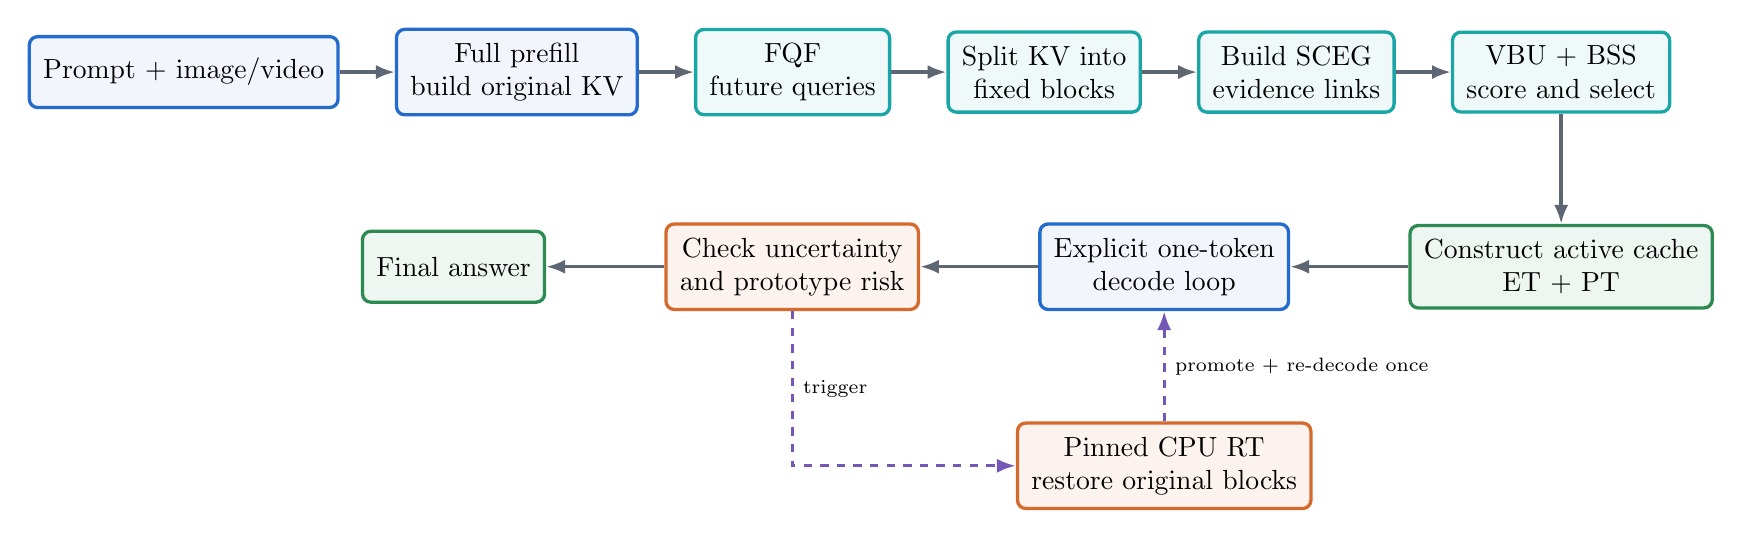
\begin{tikzpicture}[node distance=7mm and 7mm]
  \node[mainflow] (input) {Prompt + image/video};
  \node[mainflow, right=of input] (prefill) {Full prefill\\build original KV};
  \node[dataflow, right=of prefill] (forecast) {FQF\\future queries};
  \node[dataflow, right=of forecast] (blocks) {Split KV into\\fixed blocks};
  \node[dataflow, right=of blocks] (graph) {Build SCEG\\evidence links};
  \node[dataflow, right=of graph] (utility) {VBU + BSS\\score and select};

  \node[safe, below=14mm of utility] (tiers) {Construct active cache\\ET + PT};
  \node[mainflow, left=15mm of tiers] (decode) {Explicit one-token\\decode loop};
  \node[warn, left=15mm of decode] (uncertainty) {Check uncertainty\\and prototype risk};
  \node[safe, left=15mm of uncertainty] (answer) {Final answer};
  \node[warn, below=14mm of decode] (residual) {Pinned CPU RT\\restore original blocks};

  \draw[arrow] (input) -- (prefill);
  \draw[arrow] (prefill) -- (forecast);
  \draw[arrow] (forecast) -- (blocks);
  \draw[arrow] (blocks) -- (graph);
  \draw[arrow] (graph) -- (utility);
  \draw[arrow] (utility) -- (tiers);
  \draw[arrow] (tiers) -- (decode);
  \draw[arrow] (decode) -- (uncertainty);
  \draw[arrow] (uncertainty) -- (answer);
  \draw[dashedarrow] (uncertainty) |- node[tinylabel, near start, right] {trigger} (residual);
  \draw[dashedarrow] (residual) -- node[tinylabel, right] {promote + re-decode once} (decode);
\end{tikzpicture}}
\caption{The MosaicKV pipeline. One full prefill is reused; compression happens before final
token-by-token generation. Repair can bring selected source blocks back from CPU memory.}
\label{fig:overview}
\end{figure}

\why Each component fixes a different failure of simple top-$k$ pruning. Prompt attention alone
may miss future needs. Independent scores may keep duplicates. A summary may damage positional
information. A fixed compression decision may fail on a surprising future token. MosaicKV uses
forecasting, relationships, diversity, safe summaries, and repair to address these problems in
that order.

\section{Background: what the model is storing}
\label{sec:background}

\subsection{Tokens: small pieces of a larger input}

A model does not directly read a whole sentence or image. It receives a sequence of \term{tokens}.
Text tokens are word pieces. A vision encoder turns an image or video into visual features, and a
projector places those features into the language model's vector space. In the language-model
sequence, those visual features behave like many additional tokens.

For example, a document question may produce this logical sequence:

\begin{center}
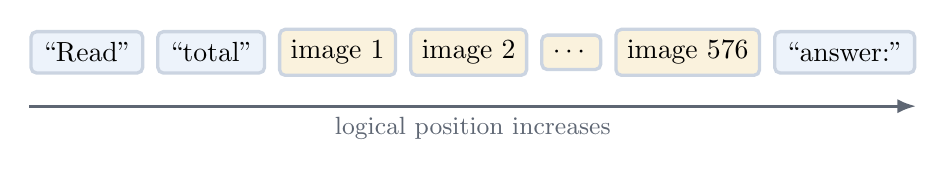
\begin{tikzpicture}[node distance=1.5mm]
  \node[memory, fill=mkblue!8] (t1) {``Read''};
  \node[memory, fill=mkblue!8, right=of t1] (t2) {``total''};
  \node[memory, fill=mkyellow!15, right=of t2] (v1) {image 1};
  \node[memory, fill=mkyellow!15, right=of v1] (v2) {image 2};
  \node[memory, fill=mkyellow!15, right=of v2] (v3) {$\cdots$};
  \node[memory, fill=mkyellow!15, right=of v3] (v4) {image 576};
  \node[memory, fill=mkblue!8, right=of v4] (t3) {``answer:''};
  \draw[arrow] ($(t1.south west)+(0,-4mm)$) -- node[below,note] {logical position increases} ($(t3.south east)+(0,-4mm)$);
\end{tikzpicture}
\end{center}

\why Visual inputs may create hundreds or thousands of language-side tokens. That makes the KV
cache much larger than it would be for a short text-only question.

\subsection{Attention, queries, keys, and values}

Attention can be explained as a search in a notebook:

\begin{itemize}
  \item A \term{query} $q$ describes what the current token is looking for.
  \item A \term{key} $k_j$ describes what stored token $j$ can be searched by.
  \item A \term{value} $v_j$ is the information returned if token $j$ is important.
\end{itemize}

For one attention head, the model computes scores and a weighted answer:

\begin{align}
  s_j &= \frac{q k_j^{\mathsf T}}{\sqrt{d}}, \\
  a_j &= \operatorname{softmax}(s)_j, \\
  o &= \sum_j a_j v_j .
\end{align}

Here $d$ is the head dimension, $a_j$ is the attention probability, and $o$ is the attention
output. A large $a_j$ means the model is looking strongly at stored token $j$ for this step.

\begin{figure}[htbp]
\centering
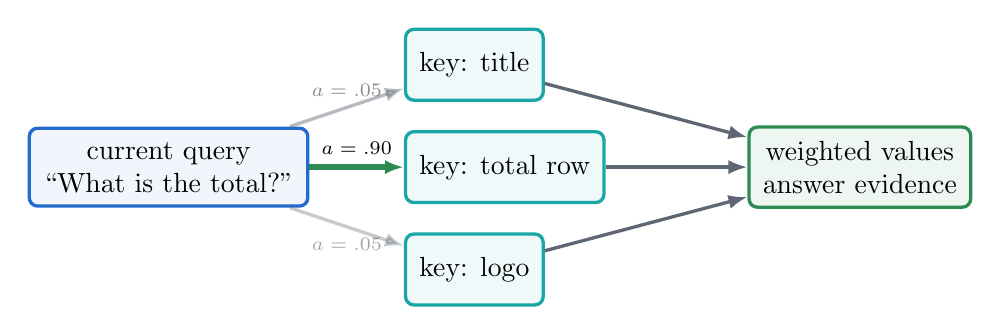
\begin{tikzpicture}[node distance=9mm and 12mm]
  \node[mainflow] (q) {current query\\``What is the total?''};
  \node[dataflow, right=of q, yshift=13mm] (k1) {key: title};
  \node[dataflow, right=of q] (k2) {key: total row};
  \node[dataflow, right=of q, yshift=-13mm] (k3) {key: logo};
  \node[safe, right=18mm of k2] (v) {weighted values\\answer evidence};
  \draw[arrow, opacity=.45] (q) -- node[above,tinylabel] {$a=.05$} (k1);
  \draw[arrow, line width=2.2pt, draw=mkgreen] (q) -- node[above,tinylabel] {$a=.90$} (k2);
  \draw[arrow, opacity=.35] (q) -- node[below,tinylabel] {$a=.05$} (k3);
  \draw[arrow] (k1) -- (v);
  \draw[arrow] (k2) -- (v);
  \draw[arrow] (k3) -- (v);
\end{tikzpicture}
\caption{A query compares with keys; the resulting probabilities mix values. This is a teaching
example, not a measurement.}
\label{fig:attention}
\end{figure}

\subsection{Why a KV cache exists}

During generation, the model produces one token at a time. Without a cache, it would recompute the
old keys and values after every new token. The KV cache stores the old K/V tensors so each step
only computes the new token's K/V.

For a common cache layout $[B,H_{KV},L,D]$:

\begin{equation}
  \text{KV bytes} = \sum_{\ell=1}^{N_{layers}}
  \left(\operatorname{bytes}(K_\ell)+\operatorname{bytes}(V_\ell)\right).
\end{equation}

For a dense, uniform cache this is approximately

\begin{equation}
  2 \times N_{layers} \times B \times H_{KV} \times L \times D
  \times \text{bytes per number}.
\end{equation}

The leading 2 counts both K and V. The length $L$ grows with text and visual tokens.

\why The cache saves computation but consumes GPU memory. Less cache memory can permit longer
inputs, more requests, or larger batches. Compression is useful only if its cost and quality loss
do not erase these benefits.

\subsection{Layers and heads: many different notebooks}

A model has many decoder layers, and a layer can have multiple KV heads. Each layer/head pair is
a separate view of the input. One head may care about words, another about nearby image regions,
and another about answer formatting.

\safety MosaicKV never combines cache entries from different layers or KV heads in one block or
prototype. Mixing them would be like combining pages from different subjects and calling the
result one page.

\section{The research problem and design goals}

MosaicKV solves this constrained problem:

\begin{quote}
Given one already-prefilled multimodal request and a hard active-KV byte budget, preserve enough
task-relevant evidence for accurate deterministic decoding, without changing model weights.
\end{quote}

The main goals are:

\begin{enumerate}
  \item \term{Quality}: retain evidence needed by future generated tokens.
  \item \term{Memory}: never exceed the configured active cache budget.
  \item \term{Correct positions}: keep the original logical position of every retained item.
  \item \term{Safety}: use an exact-only fallback when a transformation is not proven valid.
  \item \term{Auditability}: record every decision, byte, timing component, and provenance field.
  \item \term{Training-free operation}: make decisions from the current request and frozen,
        label-free calibration profiles; do not update model weights.
\end{enumerate}

MosaicKV is \emph{not} meant to change the image encoder, retrain the VLM, change tokenization, or
quietly use different prompts for different methods. Its FullKV reference performs no pruning,
merging, quantization, offloading, or repair.

\begin{plainbox}{Most important correctness gate}
At retention ratio 1.0, every source block must remain exact. No prototype or residual conversion
is allowed. The explicit decode loop must match the untouched FullKV reference within the
documented numerical tolerance. A failure blocks scientific use of that model/backend path.
\end{plainbox}

\section{End-to-end runtime}
\label{sec:runtime}

The Hugging Face MosaicKV runtime uses an explicit prefill and token-by-token decode loop. It does
not call \code{model.generate()} on the MosaicKV path. This ownership is necessary because the
cache must be inspected and possibly changed between prefill and decoding.

\begin{enumerate}
  \item Normalize messages and media with the model's processor and chat template.
  \item Run exactly one full-cache prefill. Capture K/V, query projections, and any required eager
        attention probabilities.
  \item Convert the cache to \code{FullKVState}; blockize each layer/head sequence.
  \item Forecast future queries using the existing prefill and, if configured, an isolated draft.
  \item Pool block descriptors and build the sparse evidence graph.
  \item Compute utilities and select blocks under a byte or slot budget.
  \item Build exact/prototype/residual tiers, or fail closed to exact-only mode.
  \item Pack the active cache while preserving logical positions.
  \item Decode greedily one token at a time. For full MosaicKV, evaluate repair after each
        provisional step and re-decode the same step at most once if repair triggers.
  \item Write the raw result, manifest, and debug trace, including failures.
\end{enumerate}

The following pseudocode shows ownership of the main states. It is intentionally simpler than the
Python implementation, but each named operation maps to the source files in
Section~\ref{sec:implementation-map}.

\begin{lstlisting}[style=mosaickv,language={}]
prepared = adapter.prepare_inputs(messages, media)
prefill = adapter.prefill(prepared, capture_queries=True,
                         capture_attentions=True)

full_state = blockize(adapter.extract_past_key_values(prefill),
                      logical_positions, modality_spans)
forecast, isolated_draft = forecast_with_rollout(prefill)
rope_aware_attention = pool_prompt_and_draft_attention(
    prefill, isolated_draft)

graph = build_sparse_cross_modal_evidence_graph(full_state)
utilities = compute_value_aware_block_utilities(
    graph, rope_aware_attention)
selected = lazy_greedy_select(utilities, graph, active_byte_budget)
three_tier = construct_exact_prototype_residual_tiers(
    full_state, selected, graph, adapter.prototype_key_transform)

state = pack_and_inject(three_tier, keep_logical_positions=True)
for step in decode_steps:
    provisional = adapter.decode_one_token(token, state)
    repair = maybe_restore_residuals(provisional, state)
    token, state = accept_or_redecode_once(provisional, repair)
\end{lstlisting}

\why A single owned runtime makes baselines and MosaicKV share the processor, prompt, generation
settings, byte accounting, and timing code. That makes comparisons less likely to be accidentally
unfair.

\subsection{Adapter contract}

Each model family supplies an adapter with the following operations:

\begin{longtable}{>{\raggedright\arraybackslash}p{0.30\linewidth}p{0.64\linewidth}}
\toprule
Operation & Purpose \\
\midrule
\endhead
\code{prepare_inputs(messages, media)} & Apply the correct chat template and media processor;
return tensors, modality spans, and logical length. \\
\code{prefill(...)} & Run one full prompt pass; return logits, next greedy token, cache state,
queries, and optional attentions. \\
\code{decode_one_token(...)} & Advance exactly one token using explicit logical and physical
state. \\
\code{extract_past_key_values(...)} & Snapshot model-specific cache objects without assuming a
universal type. \\
\code{inject_past_key_values(...)} & Rebuild the compatible model cache after selection or repair. \\
\code{capture_query_vectors(...)} & Hook every decoder \code{q_proj} without changing weights. \\
\code{get_modality_map(...)} & Mark text, image, and video logical spans. \\
\code{get_cache_layout(...)} & Report shapes, dtypes, devices, sequence axes, and key RoPE state. \\
\code{build_prototype_key_transform(...)} & Supply the exact model-specific phase transform, or
return unsupported. \\
\bottomrule
\end{longtable}

\why Different VLMs use different wrappers, media processors, cache classes, and position rules.
The adapter boundary keeps model-specific facts out of the generic MosaicKV algorithms.

\section{Cache state, positions, and blocks}
\label{sec:cache-state}

\subsection{Three lengths and the logical position map (LPM)}

After compression, three numbers can differ:

\begin{itemize}
  \item \term{Original logical sequence length}: how long the prompt really was.
  \item \term{Active cache length}: how many physical K/V slots remain in a packed layer/head.
  \item \term{Next decode position}: the original position assigned to the next generated token.
\end{itemize}

Suppose the original prompt positions are $0,1,2,3,4,5,6,7$, but only positions $0,2,5,7$ are
stored exactly. Their physical packed indices are $0,1,2,3$, but their logical positions remain
$0,2,5,7$. The next generated token still receives logical position 8, not 4.

\begin{figure}[htbp]
\centering
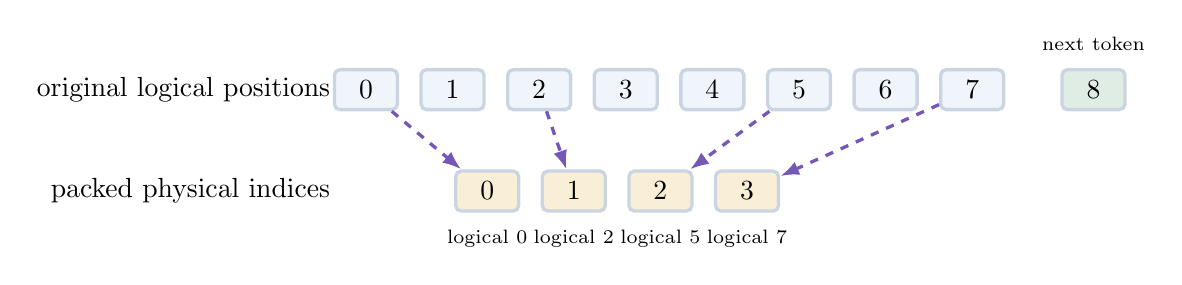
\begin{tikzpicture}[x=1.1cm,y=0.92cm]
  \node[anchor=east] at (-0.3,1.4) {original logical positions};
  \foreach \x in {0,...,7} {
    \node[memory, minimum width=8mm, fill=mkblue!7] (l\x) at (\x,1.4) {\x};
  }
  \node[memory, minimum width=8mm, fill=mkgreen!15] (next) at (8.4,1.4) {8};
  \node[above=1mm of next,tinylabel] {next token};

  \node[anchor=east] at (-0.3,0) {packed physical indices};
  \foreach \x/\logical in {0/0,1/2,2/5,3/7} {
    \node[memory, minimum width=8mm, fill=mkyellow!18] (p\x) at (\x+1.4,0) {\x};
    \node[below=1mm of p\x,tinylabel] {logical \logical};
  }
  \draw[dashedarrow] (l0) -- (p0);
  \draw[dashedarrow] (l2) -- (p1);
  \draw[dashedarrow] (l5) -- (p2);
  \draw[dashedarrow] (l7) -- (p3);
\end{tikzpicture}
\caption{Physical packing must not renumber logical positions. RoPE and the next-token position
use logical positions.}
\label{fig:positions}
\end{figure}

\why Rotary positional embeddings (RoPE) and causal attention depend on the original position.
Renumbering retained entries would change the model's meaning even if every K/V number were copied
correctly.

\how \code{LogicalPositionMap} stores physical-to-logical indices, the original sequence length,
and the next decode position. \code{DecodeState} keeps the active cache length separate from these
logical values. Packed eager caches also carry checked per-layer/head validity masks when lengths
differ.

\subsection{Fixed-size blockization}

MosaicKV usually selects groups of $b$ consecutive tokens called \term{blocks}. A block is created
inside exactly one layer and one KV head. It is also split when metadata or modality boundaries
require a separate description.

\begin{figure}[htbp]
\centering
\resizebox{0.96\textwidth}{!}{%
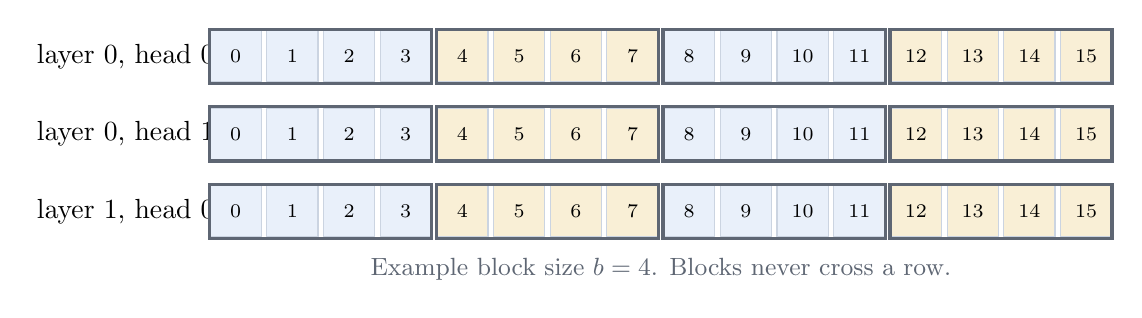
\begin{tikzpicture}[x=0.72cm,y=0.82cm]
  \node[anchor=east] at (-0.2,2.4) {layer 0, head 0};
  \node[anchor=east] at (-0.2,1.2) {layer 0, head 1};
  \node[anchor=east] at (-0.2,0.0) {layer 1, head 0};
  \foreach \row in {0,1,2} {
    \foreach \x in {0,...,15} {
      \pgfmathtruncatemacro{\start}{4*int(\x/4)}
      \pgfmathtruncatemacro{\tone}{mod(int(\x/4),2)}
      \ifnum\tone=0
        \def\fillcolor{mkblue!10}
      \else
        \def\fillcolor{mkyellow!18}
      \fi
      \node[draw=mkline, fill=\fillcolor, minimum width=6.5mm, minimum height=6.5mm,
            inner sep=0pt] at (\x,{2.4-1.2*\row}) {\scriptsize \x};
    }
  }
  \foreach \row in {0,1,2} {
    \foreach \x in {0,4,8,12} {
      \draw[very thick, draw=mkgray] (\x-0.46,{2.4-1.2*\row+0.42}) rectangle
        (\x+3.46,{2.4-1.2*\row-0.42});
    }
  }
  \node[note] at (7.5,-0.9) {Example block size $b=4$. Blocks never cross a row.};
\end{tikzpicture}}
\caption{Blockization is repeated independently for every layer and KV head.}
\label{fig:blockization}
\end{figure}

Every KV block descriptor (KVBD), implemented as \code{KVBlockDescriptor}, records:

\begin{itemize}
  \item layer, KV head, and modality;
  \item physical cache indices and original logical positions;
  \item token IDs when they exist;
  \item image, frame, page, region, OCR, or layout metadata when available;
  \item K/V dtype and device;
  \item exact byte size; and
  \item whether the block is mandatory and non-compressible.
\end{itemize}

\why Blocks reduce the number of decisions. Selecting token-by-token can be expensive and may
break nearby evidence into tiny pieces. Fixed-size blocks also make a cardinality budget useful.
The byte-budget path remains available for short final blocks or variable representations.

\safety Every source cache position belongs to exactly one block for its layer/head. Positions
inside a block must be strictly increasing. Mandatory tokens can never be removed.

\section{Component 1: future-query forecasting (FQF)}
\label{sec:forecast}

The prefill tells us what the prompt looked at, but generation may ask for different evidence.
MosaicKV therefore estimates what future decoder queries may look like before it compresses the
cache.

\subsection{Three forecasting modes}

\paragraph{Prompt-window (PW) mode.} Use query projections and attention from the last $w$ prompt
positions. The end of a question often says what kind of answer is needed.

\why This mode is cheap because the queries already exist after prefill. Its weakness is that the
prompt's own queries may not match the queries created after the model starts answering.

\paragraph{Draft-rollout (DR) mode.} Start from the original prefill, clone its decode state, run $r$
temporary greedy tokens with the full cache, and capture their queries and attention. Then discard
the draft tokens and cloned cache.

\why Draft queries are closer to real future decoding. They cost extra time, so $r$ must remain
small. Reusing the original prefill avoids performing the expensive image and prompt work twice.

\paragraph{Hybrid query forecast (HQF) mode.} Combine PW statistics with DR queries. Stable heads can
lean on prompt evidence, while heads whose prompt and draft attention distributions differ can
lean more strongly on the draft.

\why The prompt is a safe anchor and the draft captures future change. Combining them reduces the
risk of trusting only one imperfect signal.

\begin{figure}[htbp]
\centering
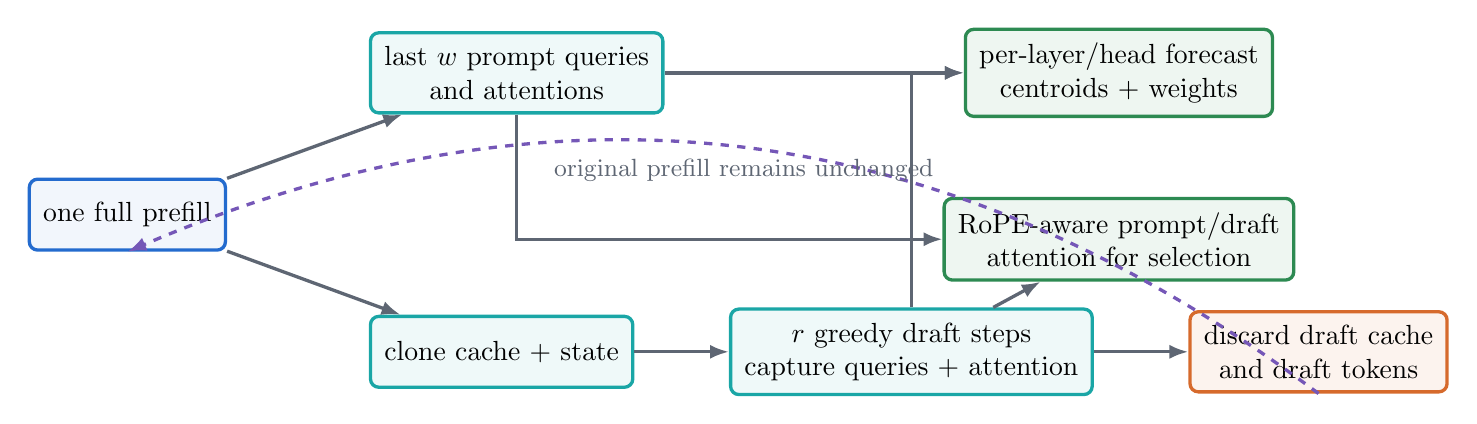
\begin{tikzpicture}[node distance=7mm and 12mm]
  \node[mainflow] (prefill) {one full prefill};
  \node[dataflow, above right=8mm and 18mm of prefill] (prompt) {last $w$ prompt queries\\and attentions};
  \node[dataflow, below right=8mm and 18mm of prefill] (clone) {clone cache + state};
  \node[dataflow, right=of clone] (draft) {$r$ greedy draft steps\\capture queries + attention};
  \node[warn, right=of draft] (discard) {discard draft cache\\and draft tokens};
  \node[safe, right=38mm of prompt] (forecast) {per-layer/head forecast\\centroids + weights};
  \node[safe, below=10mm of forecast] (attention) {RoPE-aware prompt/draft\\attention for selection};
  \draw[arrow] (prefill) -- (prompt);
  \draw[arrow] (prefill) -- (clone);
  \draw[arrow] (clone) -- (draft);
  \draw[arrow] (draft) -- (discard);
  \draw[arrow] (prompt) -- (forecast);
  \draw[arrow] (draft) |- (forecast);
  \draw[arrow] (prompt) |- (attention);
  \draw[arrow] (draft) -- (attention);
  \draw[dashedarrow] (discard.south) to[bend right=30] node[below,note]
    {original prefill remains unchanged} (prefill.south);
\end{tikzpicture}
\caption{Forecasting reuses one prefill. Query vectors build the forecast object; actual eager
attention supplies position-aware online block evidence.}
\label{fig:forecast}
\end{figure}

\subsection{The query forecast (QF) object}

For every layer and KV head, the QF type \code{QueryForecast} stores:

\begin{itemize}
  \item prompt mean $\mu$;
  \item full covariance $\Sigma$ or diagonal variance;
  \item draft query samples;
  \item normalized query centroids $c_1,\ldots,c_K$;
  \item weights $\pi_1,\ldots,\pi_K$ that sum to one; and
  \item provenance saying which prompt positions and query heads were used.
\end{itemize}

Grouped-query attention (GQA) is handled explicitly. If several query heads share one KV head, their
queries become samples for that KV head instead of being silently dropped.

The low-memory centroid path uses a deterministic streaming spherical update. Its extra centroid
memory is $O(KD)$ rather than storing a large sample-by-centroid matrix.

\subsection{Why query vectors are not directly dotted with cached keys}

The current model hooks capture \code{q_proj} output \emph{before} RoPE. Supported model caches
store keys \emph{after} RoPE. A direct dot product would compare two different coordinate systems.
The online runtime therefore pools actual eager prompt/draft attention probabilities, which
already contain the model's correct positional transformation. The query centroids remain useful
for forecast statistics, diagnostics, and future audited transforms.

\safety Pre-RoPE query vectors are never silently multiplied by post-RoPE keys and labeled valid
attention. Any attention supplied to utility computation must explicitly declare RoPE-aware
provenance.

\subsection{Forecast diagnostics}

The evaluation-only oracle path collects true future queries from a cloned FullKV decode. It
reports:

\begin{itemize}
  \item cosine similarity to true future queries;
  \item Spearman rank correlation between predicted and true attention;
  \item recall of blocks chosen by an oracle future-attention ranking; and
  \item forecast regret, the true attention mass missed relative to the oracle selection.
\end{itemize}

\why These metrics tell us whether a forecast is useful even when the final answer happens to be
correct by chance. The oracle is isolated in an evaluation namespace and never enters the online
compressor.

\section{Component 2: sparse cross-modal evidence graph (SCEG)}
\label{sec:graph}

A visual answer often depends on a group of related pieces. In a chart, a legend color, a bar,
and its axis label may be far apart in token order. In a document, a table cell and its row header
may form one fact. MosaicKV models these relationships with a graph.

Each node is one KV block. A graph edge says, ``these blocks may support the same evidence.'' The
edge has a type and a configurable weight.

\begin{figure}[htbp]
\centering
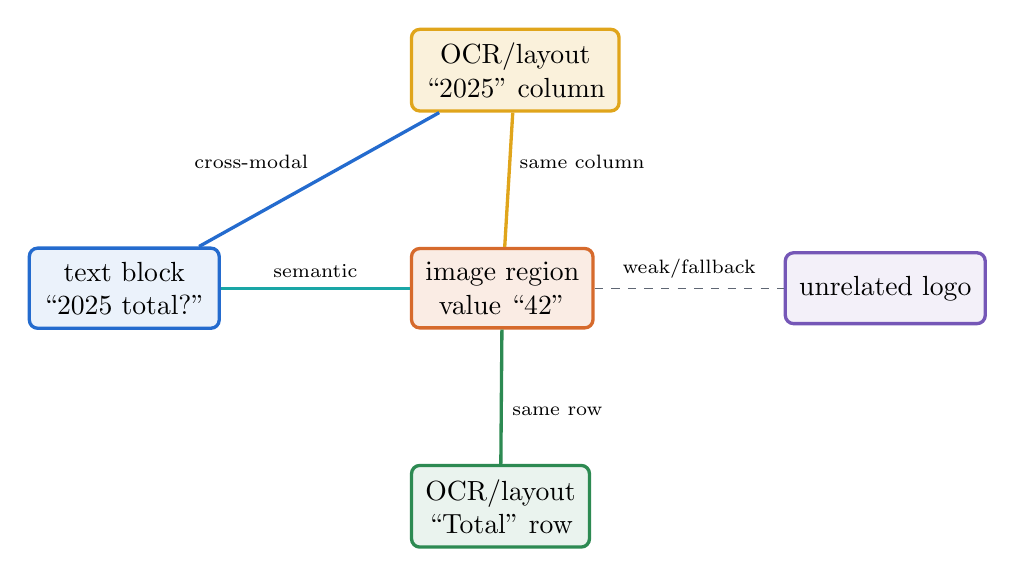
\begin{tikzpicture}[node distance=17mm and 24mm]
  \node[flow, draw=mkblue, fill=mkblue!9] (question) {text block\\``2025 total?''};
  \node[flow, draw=mkyellow, fill=mkyellow!16, above right=of question] (header) {OCR/layout\\``2025'' column};
  \node[flow, draw=mkorange, fill=mkorange!13, right=of question] (cell) {image region\\value ``42''};
  \node[flow, draw=mkgreen, fill=mkgreen!10, below right=of question] (row) {OCR/layout\\``Total'' row};
  \node[flow, draw=mkpurple, fill=mkpurple!9, right=of cell] (logo) {unrelated logo};
  \draw[very thick, draw=mkblue] (question) -- node[above left,tinylabel] {cross-modal} (header);
  \draw[very thick, draw=mkyellow] (header) -- node[above right,tinylabel] {same column} (cell);
  \draw[very thick, draw=mkgreen] (row) -- node[below right,tinylabel] {same row} (cell);
  \draw[very thick, draw=mkcyan] (question) -- node[above,tinylabel] {semantic} (cell);
  \draw[dashed, draw=mkgray] (cell) -- node[above,tinylabel] {weak/fallback} (logo);
\end{tikzpicture}
\caption{A teaching example of cross-modal evidence connections. Edge types remain separate, so
one source can be disabled without breaking the others.}
\label{fig:graph-example}
\end{figure}

\subsection{Block descriptors used by the graph}

For each block, the graph builder pools:

\begin{itemize}
  \item a key descriptor;
  \item a value descriptor;
  \item an optional hidden-state descriptor;
  \item optional prompt-attention co-activation; and
  \item media, OCR, layout, region, page, frame, and bounding-box metadata.
\end{itemize}

Pooling changes a small group of token vectors into a compact block vector. It does not change the
actual K/V cache. These descriptors are used only for scoring relationships.

\why Comparing full K/V tensors for every graph decision would be slow and memory hungry. Pooled
descriptors provide a smaller search representation while exact tensors remain available for
construction.

\subsection{Edge types}

\begin{longtable}{>{\raggedright\arraybackslash}p{0.23\linewidth}p{0.46\linewidth}p{0.24\linewidth}}
\toprule
Edge type & What it means & Why it helps \\
\midrule
\endhead
Semantic similarity & Pooled descriptors point in similar directions. & Finds evidence with
similar meaning even when positions are far apart. \\
Prompt attention co-activation & Prompt queries looked at both blocks in a similar pattern. &
Connects items the model already used together. \\
Spatial adjacency & Normalized image boxes are near or touching. & Preserves neighboring chart,
diagram, and object regions. \\
OCR/layout & Same OCR text, row, column, reading order, or page region. & Connects document and
table structure. \\
Temporal adjacency & Frame or clip indices are within a configured window. & Preserves local
events in a video. \\
Same evidence region & Metadata assigns blocks to the same region identifier. & Keeps pieces of a
single detected fact together. \\
Cross-modal alignment & Related blocks use different modalities, such as question text and image
region. & Joins what was asked with where the answer may appear. \\
Fallback & Nearby compatible blocks are connected when rich metadata is absent. & Keeps the
algorithm usable without inventing unavailable layout facts. \\
\bottomrule
\end{longtable}

\subsection{Compatibility filters}

Before any edge is added, both nodes must pass configured filters:

\begin{itemize}
  \item same layer, unless an experiment explicitly disables this requirement;
  \item same KV head, unless explicitly disabled;
  \item an allowed directed modality pair, such as \code{text:image}; and
  \item a maximum logical-position span for edge types that require locality.
\end{itemize}

Spatial edges use normalized image coordinates. Temporal edges use actual frame/clip indices.
Layout edges use metadata only when it exists. Missing metadata activates a labeled fallback; it
does not fabricate OCR boxes or frame identities.

\subsection{Keeping the graph sparse}

A dense graph for $n$ blocks can have $n^2$ pair scores. MosaicKV limits each node and edge source
to its top $d$ neighbors. Semantic and attention similarity are computed in chunks, so the normal
path materializes only a chunk-by-candidate tile, not a full $n\times n$ matrix. Spatial lookup
uses grid buckets; layout and temporal sources use bounded local groups. Storage uses sparse COO
arrays and can be converted to CSR.

With fixed $d$, stored graph memory is $O(nd)$.

\why Sparse storage matters because graph construction must save memory, not become a new memory
problem. Separate typed edges also make ablations honest: turning off spatial edges does not
silently remove semantic or temporal edges.

\subsection{Graph diagnostics}

The trace records node and edge counts, average degree, connected components, modality mixing,
edge-source counts, and evidence-cluster coverage. These values help detect an empty graph, an
over-connected graph, or metadata that was not loaded as expected.

\section{Component 3: value-aware block utility (VBU)}
\label{sec:utility}

The sparse cross-modal evidence graph (SCEG) says how blocks relate. Value-aware block utility
(VBU) says how useful each block may be. A useful block can matter for several different reasons,
so VBU keeps the signals separate before combining them.

\subsection{The seven recorded signals}

For block $i$, the implementation records:

\begin{enumerate}
  \item \term{Forecast attention probability} $p_i$: predicted attention mass on the block,
        normalized inside its layer/KV-head group.
  \item \term{Value novelty} $n_i$: one minus the largest positive cosine similarity between its
        pooled value and a graph neighbor's value.
  \item \term{Expected attention-output contribution} $c_i$: forecast probability multiplied by
        the pooled value-vector norm, then normalized inside the layer/head group.
  \item \term{Graph centrality and singleton coverage}: how much of the SCEG this block can
        represent by itself.
  \item \term{Modality rarity}: whether its modality is uncommon in this request's graph.
  \item \term{Redundancy penalty}: the complement of value novelty.
  \item \term{Mandatory priority}: one for mandatory blocks and zero otherwise.
\end{enumerate}

\begin{figure}[htbp]
\centering
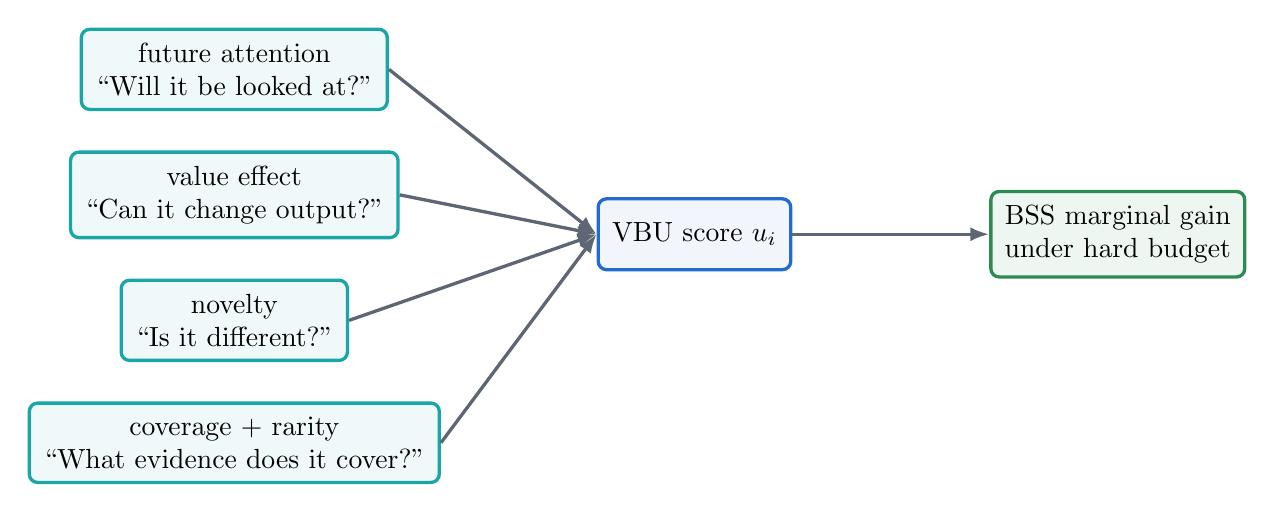
\begin{tikzpicture}[node distance=5mm and 13mm]
  \node[dataflow] (attn) {future attention\\``Will it be looked at?''};
  \node[dataflow, below=of attn] (value) {value effect\\``Can it change output?''};
  \node[dataflow, below=of value] (novel) {novelty\\``Is it different?''};
  \node[dataflow, below=of novel] (graph) {coverage + rarity\\``What evidence does it cover?''};
  \node[mainflow, right=25mm of value, yshift=-5mm] (score) {VBU score $u_i$};
  \node[safe, right=25mm of score] (selector) {BSS marginal gain\\under hard budget};
  \draw[arrow] (attn.east) -- (score.west);
  \draw[arrow] (value.east) -- (score.west);
  \draw[arrow] (novel.east) -- (score.west);
  \draw[arrow] (graph.east) -- (score.west);
  \draw[arrow] (score) -- (selector);
\end{tikzpicture}
\caption{VBU does not treat attention as the only definition of importance.}
\label{fig:utility}
\end{figure}

\why Attention-only selection can keep blocks that are frequently viewed but interchangeable,
or miss a low-attention block with a large, unique value vector. VBU asks both ``will it be
looked at?'' and ``what happens if it is used?''

\subsection{Local utility equation}

The registered local utility is implemented literally:

\begin{equation}
  u_i = \lambda_q p_i - \lambda_v c_i - \lambda_o n_i .
  \label{eq:local-utility}
\end{equation}

The minus signs are part of the system contract. Therefore, a negative $\lambda_v$ or
$\lambda_o$ turns the corresponding term into a preservation reward. The default configuration
uses $\lambda_q=1$, $\lambda_v=-0.25$, and $\lambda_o=-0.25$. With those signs,
Equation~\ref{eq:local-utility} becomes attention plus smaller rewards for contribution and
novelty.

\begin{plainbox}{Why the sign explanation matters}
If a reader saw the minus signs but assumed all $\lambda$ values were positive, it would appear
that MKV intentionally dislikes valuable or unique evidence. The coefficients are signed and are
stored in every resolved configuration, so the exact behavior can be audited.
\end{plainbox}

Attention, contribution, and novelty are each nonnegative and normalized to sum to one inside
every layer/KV-head stratum. This keeps a coefficient from changing meaning merely because one
prompt contains more visual tokens.

\subsection{Prompt anchors and fine evidence preservation}

Two optional hard reservations act as quality guards before ordinary greedy choice:

\begin{itemize}
  \item A \term{prompt-anchor reservation (PAR)} keeps a configured fraction of blocks with the
        strongest prompt-only attention.
  \item An \term{evidence-preservation reservation (EPR)} keeps a configured fraction of blocks
        with strong SCEG evidence scores.
\end{itemize}

Both reservations consume the same active budget; they are not free extra memory. Each selected
block receives a distinct reason in the trace.

\why A forecast can be wrong. PAR retains a small amount of direct prompt evidence as a safety
anchor. EPR protects fine chart/document structure that a broad semantic score could otherwise
replace with a nearby but incorrect region.

\section{Component 4: budgeted submodular selection (BSS)}
\label{sec:selection}

After VBU scores blocks, budgeted submodular selection (BSS) chooses a set $S$. ``Submodular'' is a
formal version of the idea that the first useful representative helps more than a tenth similar
representative. In plain language, BSS tries to keep useful \emph{and diverse} blocks.

\subsection{The set objective}

MosaicKV uses this registered objective:

\begin{equation}
  F(S)=\sum_{i\in S}u_i
  -\lambda_g C_{FL}(S)
  -\lambda_m C_{mod}(S),
  \label{eq:set-objective}
\end{equation}

where:

\begin{itemize}
  \item $C_{FL}(S)$ is facility-location (FL) coverage: for each graph node, use the largest
        similarity supplied by any selected representative, and then average;
  \item $C_{mod}(S)$ is modality coverage: the fraction of available modalities represented in
        $S$.
\end{itemize}

Like the local equation, Equation~\ref{eq:set-objective} uses literal minus signs. Coverage is a
reward when $\lambda_g\leq0$ and $\lambda_m\leq0$. The default values are both $-0.25$. Those signs
preserve the diminishing-returns condition used by the lazy-greedy proof. Positive values turn
coverage into a penalty; exact objective evaluation still works, but the lazy selector rejects
that configuration.

\why Adding FL and modality coverage discourages the selector from spending most of its budget on
near-duplicates from one region or modality.

\subsection{Hard budget units}

The selector supports three budget units:

\begin{itemize}
  \item \term{blocks}: each fixed-size block costs one;
  \item \term{retained slots}: a block costs its number of source positions; and
  \item \term{bytes}: a block costs its exact K/V payload bytes.
\end{itemize}

Paper comparisons must use active KV bytes as the primary budget. A nominal retention percentage
is not comparable when two methods count different layers, heads, dtypes, tiers, or metadata.

For a byte-matched MKV run, the requested retention ratio (RR) is

\begin{equation}
  \rho_{request}=\frac{\text{target active KV bytes}}
  {\text{FullKV prompt KV bytes}}.
\end{equation}

The physical cache may require whole blocks or a common dense length, so the realized ratio is

\begin{equation}
  \rho_{real}=\frac{\text{measured packed ET + PT bytes}}
  {\text{measured FullKV prompt KV bytes}}.
\end{equation}

The result row records both. Scientific comparison uses $\rho_{real}$ and the underlying byte
counts. Sweeping several RRs reveals the quality--memory curve: a method that works only at one
large budget may not work at a tighter budget.

\safety Mandatory exact blocks are selected first. If they alone exceed the budget, MKV stops
with an error rather than silently violating the budget. The final selected active cost can never
exceed the configured limit.

Mandatory blocks are determined before method-specific ranking. In the ordinary MKV path, the
last prompt position is mandatory because it is the immediate generation boundary. A baseline
with a paper-defined protected prefix/suffix may require additional mandatory positions, but this
difference must be reported rather than hidden.

\subsection{Lazy greedy in simple steps}

\begin{enumerate}
  \item Insert mandatory blocks in deterministic node order.
  \item Insert required PAR, EPR, and PT-anchor blocks, each with a recorded reason.
  \item For each remaining block, compute marginal gain
        $\Delta(i\mid S)=F(S\cup\{i\})-F(S)$.
  \item Put candidates in a priority queue ordered by gain per cost.
  \item Pop the best candidate. If its cached gain is stale because $S$ changed, recompute it and
        return it to the queue.
  \item Select it only if it fits the remaining budget and passes physical-capacity constraints.
  \item Repeat until the budget is full or all remaining gains are nonpositive.
\end{enumerate}

\begin{figure}[htbp]
\centering
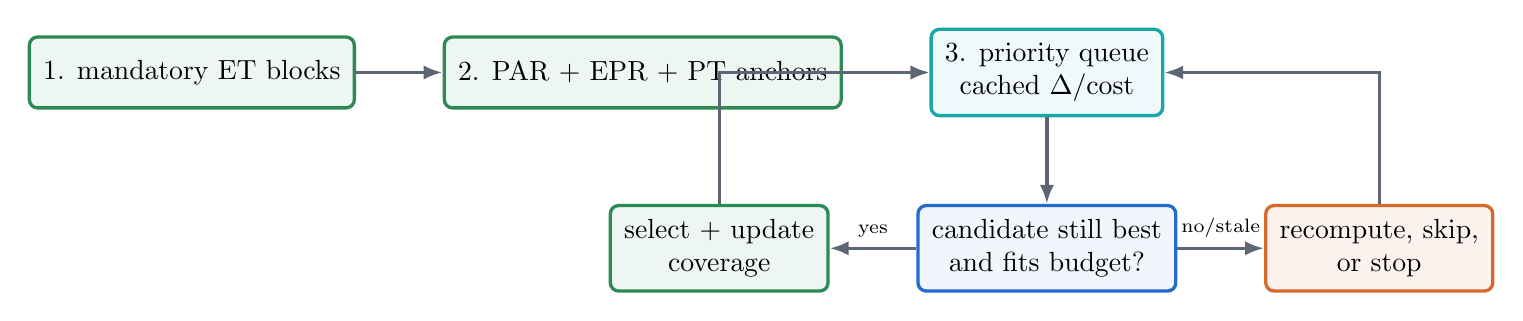
\begin{tikzpicture}[node distance=7mm and 11mm]
  \node[safe] (mandatory) {1. mandatory ET blocks};
  \node[safe, right=of mandatory] (guards) {2. PAR + EPR + PT anchors};
  \node[dataflow, right=of guards] (heap) {3. priority queue\\cached $\Delta/$cost};
  \node[mainflow, below=11mm of heap] (check) {candidate still best\\and fits budget?};
  \node[safe, left=of check] (keep) {select + update\\coverage};
  \node[warn, right=of check] (skip) {recompute, skip,\\or stop};
  \draw[arrow] (mandatory) -- (guards);
  \draw[arrow] (guards) -- (heap);
  \draw[arrow] (heap) -- (check);
  \draw[arrow] (check) -- node[above,tinylabel] {yes} (keep);
  \draw[arrow] (check) -- node[above,tinylabel] {no/stale} (skip);
  \draw[arrow] (keep) |- (heap);
  \draw[arrow] (skip) |- (heap);
\end{tikzpicture}
\caption{Deterministic lazy-greedy BSS. Cached gains avoid recomputing every candidate after every
selection.}
\label{fig:lazy-greedy}
\end{figure}

Ties are deterministic: larger gain density, larger raw gain, lower cost, then lower node ID.
Every block receives a decision record, including rejected blocks.

\why Ordinary greedy recomputation can be expensive. Lazy greedy exploits diminishing returns:
an old marginal gain is an upper bound until the candidate is reconsidered.

\subsection{Tiny exhaustive solver}

For small synthetic graphs, the implementation enumerates every feasible subset and finds the
best objective exactly. It compares the greedy set with this optimum and reports the absolute and
relative gap. A separate property audit checks monotonicity and diminishing returns.

\why The exhaustive solver is too expensive for normal graphs, but it is a strong correctness
test for the selector and objective formula.

\section{Component 5: the three-tier cache (TTC)}
\label{sec:tiers}

The three-tier cache (TTC) represents selected and unselected information in three different ways.
Only the exact tier (ET) and prototype tier (PT) are active language-model KV on the graphics
processing unit (GPU). The residual tier (RT) is host-side recovery data on the central processing
unit (CPU).

\begin{figure}[htbp]
\centering
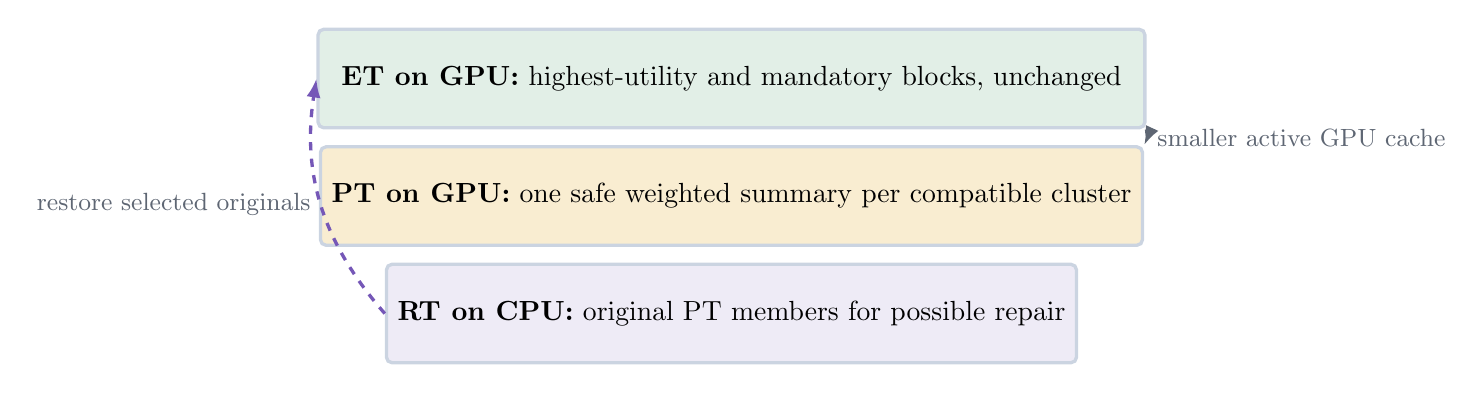
\begin{tikzpicture}[node distance=2mm]
  \node[memory, fill=mkgreen!14, minimum width=10.5cm, minimum height=1.25cm] (exact)
    {\textbf{ET on GPU:} highest-utility and mandatory blocks, unchanged};
  \node[memory, fill=mkyellow!20, minimum width=8.7cm, minimum height=1.25cm,
        below=of exact] (proto)
    {\textbf{PT on GPU:} one safe weighted summary per compatible cluster};
  \node[memory, fill=mkpurple!12, minimum width=7.0cm, minimum height=1.25cm,
        below=of proto] (residual)
    {\textbf{RT on CPU:} original PT members for possible repair};
  \draw[arrow] (exact.south east) to[bend left=16] node[right,note] {smaller active GPU cache} (proto.north east);
  \draw[dashedarrow] (residual.west) to[bend left=25] node[left,note] {restore selected originals} (exact.west);
\end{tikzpicture}
\caption{The TTC. RT bytes are recorded separately and are never hidden inside the active-GPU
budget.}
\label{fig:tiers}
\end{figure}

\subsection{Exact tier (ET)}

The ET gathers selected blocks without changing their numbers, dtype, logical positions, or
metadata. It may alias or copy storage depending on the safe runtime path.

\why The most important evidence should not pay an approximation error. Mandatory prompt tokens
also need an unchanged causal and positional reference.

\safety At retention 1.0, every source block goes to ET. PT and RT must be empty, and exact
reinjection must reconstruct the original cache bit for bit.

\subsection{Prototype tier (PT)}

For each unselected block, MKV searches for the highest-weight compatible selected anchor. An
anchor must be in the same layer and KV head, use an allowed modality direction, and stay within
the configured logical-position span. The selected anchor remains exact; it identifies the
cluster and the logical position of its prototype.

If a PT cluster contains source members $j=1,\ldots,m$ with positive raw weights $w_j$, normalized
weights are

\begin{equation}
  \alpha_j=\frac{w_j}{\sum_{r=1}^{m}w_r}.
\end{equation}

After safe position handling, the prototype values are computed in 32-bit floating point (FP32):

\begin{align}
  \bar{k} &= \sum_{j=1}^{m}\alpha_j\,\operatorname{pool}(k_j), \\
  \bar{v} &= \sum_{j=1}^{m}\alpha_j\,\operatorname{pool}(v_j).
\end{align}

The result uses one active cache slot and is cast back to the cache dtype and device.

\why Some unselected blocks contain similar evidence. A prototype preserves a summary inside the
active budget instead of discarding all of them. This can improve quality at the same active
memory only when the summary is positionally and numerically safe.

\subsection{RoPE-safe prototype keys}

Rotary position embedding (RoPE) rotates key/query dimensions according to logical position.
Supported caches store keys after this rotation. Averaging two post-RoPE keys at different
positions is like averaging two arrows after rotating the paper underneath them: the result mixes
content with incompatible angles.

The audited prototype key transform (PKT) performs three steps:

\begin{enumerate}
  \item invert each source member's exact RoPE phase to recover phase-neutral content;
  \item pool and compute the weighted FP32 mean in phase-neutral space; and
  \item apply the selected anchor's exact RoPE phase to create the cache-ready prototype key.
\end{enumerate}

\begin{figure}[htbp]
\centering
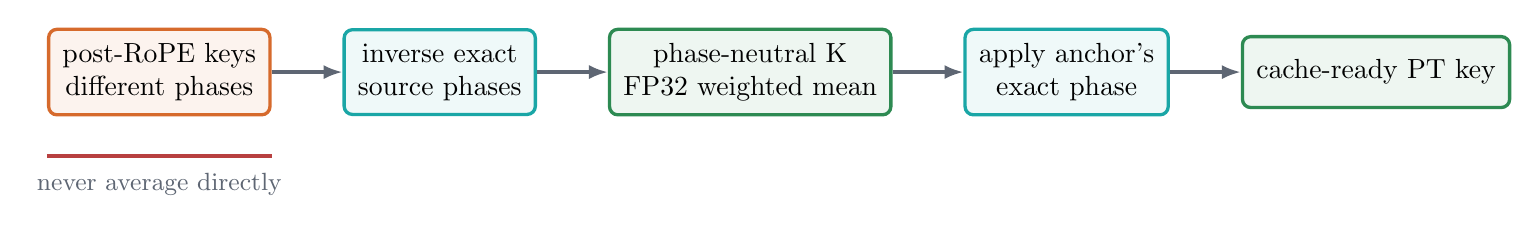
\begin{tikzpicture}[node distance=7mm and 9mm]
  \node[warn] (post) {post-RoPE keys\\different phases};
  \node[dataflow, right=of post] (inverse) {inverse exact\\source phases};
  \node[safe, right=of inverse] (neutral) {phase-neutral K\\FP32 weighted mean};
  \node[dataflow, right=of neutral] (anchor) {apply anchor's\\exact phase};
  \node[safe, right=of anchor] (ready) {cache-ready PT key};
  \draw[arrow] (post) -- (inverse);
  \draw[arrow] (inverse) -- (neutral);
  \draw[arrow] (neutral) -- (anchor);
  \draw[arrow] (anchor) -- (ready);
  \draw[very thick, draw=mkred] ($(post.south west)+(0,-5mm)$) -- ($(post.south east)+(0,-5mm)$);
  \node[below=6mm of post,note] {never average directly};
\end{tikzpicture}
\caption{RoPE-safe key merging. Qwen2.5-VL uses multimodal RoPE (M-RoPE); LLaVA families use
their audited standard RoPE phases.}
\label{fig:rope}
\end{figure}

For Qwen2.5-VL, the PKT uses the model's temporal, height, and width M-RoPE phases. For LLaVA-1.5
and LLaVA-OneVision, it uses the exact standard Llama/Qwen2 phase for an unpadded monotonic request.
The implementation is pinned to Hugging Face Transformers 4.55.2 for these transforms.

\safety If the adapter, version, cache key state, position layout, or transform provenance does
not match the audited rule, PT is disabled. The run becomes an explicitly labeled exact-only
safety fallback; it is never presented as successful prototype MKV.

\subsection{Adaptive grouping and per-head routing}

Not every KV head tolerates the same amount of averaging. A label-free calibration path compares
exact selection with prototype reconstruction for each layer/head. Sensitive heads can be routed
to:

\begin{itemize}
  \item ET only;
  \item a smaller maximum PT group size; or
  \item a shorter maximum logical-position span.
\end{itemize}

Optional member-level key/value error and cluster-dispersion limits reject damaging groups before
materialization. Prototype weights can also include future-attention importance rather than using
only graph strength.

\why A global prototype size treats all heads as equally robust. Per-head routing spends exact
memory where approximation is most harmful and uses stronger compression where it is safer.

\subsection{Prototype diagnostics}

Every prototype record stores its anchor, member IDs, raw/normalized weights, modality
composition, logical-position span, K/V mean-squared error (MSE) dispersion, member bytes,
prototype bytes, active bytes saved, per-member reconstruction error, and anchor selection
utility.

\why These diagnostics allow a failed answer or repair event to be traced back to the exact
cluster that may have caused it.

\subsection{Residual tier (RT)}

The RT preserves original source blocks represented by PT. It is indexed by layer, KV head,
prototype ID, original logical position, and source position. The default representation is
lossless. Optional 16-bit floating point (FP16), brain floating point (BF16), 8-bit floating point
(FP8), and symmetric 8-bit integer (INT8) encodings are available for controlled experiments.

Lossless Torch RT payloads use contiguous pinned CPU slabs. Pinned memory allows asynchronous
CPU-to-GPU transfer on a dedicated CUDA stream. If production configuration requires pinned
memory and it is unavailable, construction fails instead of pretending repair is ready.

\why PT is an approximation. RT provides a reversible path for the small number of moments when
that approximation appears dangerous. Keeping it on the CPU saves active GPU memory, but its
bytes and transfer cost are still reported separately.

\section{Component 6: uncertainty-guided residual repair (UGRR)}
\label{sec:repair}

Uncertainty-guided residual repair (UGRR) observes each provisional decode step. It does not know
the correct answer online. It uses uncertainty and prototype evidence to decide whether restoring
a few original blocks may be worthwhile.

\subsection{Signals computed at a provisional step}

Let $p$ be the softmax probability distribution over the vocabulary of size $|\mathcal V|$.
Normalized next-token entropy is

\begin{equation}
  H_{norm}=-\frac{\sum_x p_x\log p_x}{\log |\mathcal V|},
  \qquad 0\le H_{norm}\le1.
\end{equation}

High entropy means the model spreads probability over many possible tokens.

For prototype $j$, let $A_j$ be its globally normalized current attention mass and $D_j$ its
average K/V dispersion. Raw prototype risk is

\begin{equation}
  R_j=A_jD_j.
\end{equation}

The implementation can normalize risks to sum to one for a calibrated decision-aware repair (DAR)
profile. It also computes the probability margin between the two most likely next tokens. A small
margin means a modest logit change could flip the decision. An optional Kullback--Leibler (KL)
divergence from a cheap draft distribution is recorded as a diagnostic.

\why Entropy alone may trigger even when no prototype is responsible. Prototype risk alone may
trigger when the model is highly confident. Combining risk with a low decision margin targets
steps where prototype approximation is both relevant and capable of changing the token.

\subsection{Repair policies}

\begin{longtable}{>{\bfseries}p{0.25\linewidth}p{0.66\linewidth}}
\toprule
Policy & Rule \\
\midrule
\endhead
none & Never trigger. This is the required control. \\
entropy & Trigger when $H_{norm}$ reaches its configured threshold. \\
prototype risk & Trigger when $\max_j R_j$ reaches its threshold and any minimum-entropy guard. \\
entropy or prototype risk & Trigger when either of the two previous rules is true. \\
decision aware & Trigger for very high normalized risk, or for moderate risk plus a sufficiently
small next-token probability margin. \\
oracle & Evaluation-only counterfactual trigger using a FullKV reference decision. It is forbidden
in the online compressor. \\
\bottomrule
\end{longtable}

\subsection{What happens after a trigger}

\begin{enumerate}
  \item Rank active prototype clusters by current risk, with prototype ID as the tie-breaker.
  \item Rank their RT members by configured importance. The default uses normalized member weight
        times reconstruction error; decision-influence mode also includes value-output norm.
  \item Choose at most $R$ original residual blocks, spreading early choices across high-risk
        clusters.
  \item Plan budget effects before transfer. If necessary, evict the lowest-utility non-protected
        prototype.
  \item Transfer chosen originals from pinned CPU memory, restore their source dtype/device, and
        promote them permanently to ET.
  \item If only part of a prototype was restored, algebraically refresh the remaining PT mean and
        dispersion; do not throw away unpromoted members.
  \item Rebuild/reinject the active cache and recompute the \emph{same} token exactly once.
  \item Keep promoted blocks for later decode steps and record the entire event.
\end{enumerate}

\begin{figure}[htbp]
\centering
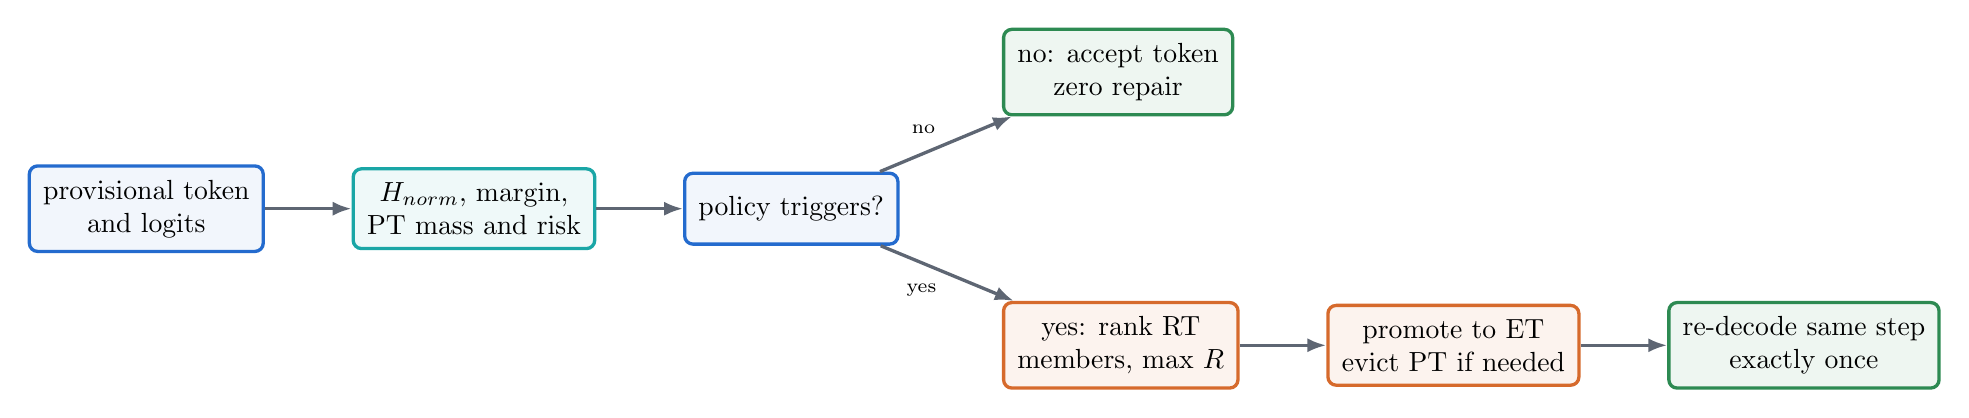
\begin{tikzpicture}[node distance=6mm and 11mm]
  \node[mainflow] (provisional) {provisional token\\and logits};
  \node[dataflow, right=of provisional] (signals) {$H_{norm}$, margin,\\PT mass and risk};
  \node[mainflow, right=of signals] (trigger) {policy triggers?};
  \node[safe, above right=7mm and 13mm of trigger] (accept) {no: accept token\\zero repair};
  \node[warn, below right=7mm and 13mm of trigger] (rank) {yes: rank RT\\members, max $R$};
  \node[warn, right=of rank] (budget) {promote to ET\\evict PT if needed};
  \node[safe, right=of budget] (redecode) {re-decode same step\\exactly once};
  \draw[arrow] (provisional) -- (signals);
  \draw[arrow] (signals) -- (trigger);
  \draw[arrow] (trigger) -- node[above left,tinylabel] {no} (accept);
  \draw[arrow] (trigger) -- node[below left,tinylabel] {yes} (rank);
  \draw[arrow] (rank) -- (budget);
  \draw[arrow] (budget) -- (redecode);
\end{tikzpicture}
\caption{UGRR is a bounded transaction. One event can recompute the current token at most once.}
\label{fig:repair}
\end{figure}

\safety A plan that cannot fit the active budget performs no transfer and records
\code{active_budget_infeasible}. The same step cannot be repaired twice. Policy \code{none} never
triggers. Online code cannot receive oracle decisions or FullKV reference tokens.

\subsection{Decision-aware repair calibration}

A label-free calibration ledger can compare compressed provisional tokens with FullKV tokens on
disjoint calibration examples. It searches moderate-risk, high-risk, and decision-margin
thresholds under a registered maximum trigger rate and minimum repair precision. It uses no task
answer labels.

If no threshold set passes the precision and trigger-rate gates, the frozen profile disables
repair and predicts zero online triggers.

\why An uncalibrated repair rule can make correct answers worse or spend too much latency. Failing
closed is better than enabling a rule that did not meet its preregistered evidence threshold.

\section{How the six components work together}
\label{sec:why-combination}

The components are ordered because each one supplies information or safety needed by the next:

\begin{enumerate}
  \item FQF says what future decoding may need.
  \item SCEG says which pieces form shared evidence.
  \item VBU says which individual blocks are useful and nonredundant.
  \item BSS converts those signals into a diverse set that fits a hard budget.
  \item TTC preserves selected evidence exactly, summarizes compatible omissions, and keeps a
        recovery copy outside active GPU memory.
  \item UGRR reacts when a specific future token reveals that the fixed compression decision was
        unsafe.
\end{enumerate}

\begin{figure}[htbp]
\centering
\resizebox{0.98\textwidth}{!}{%
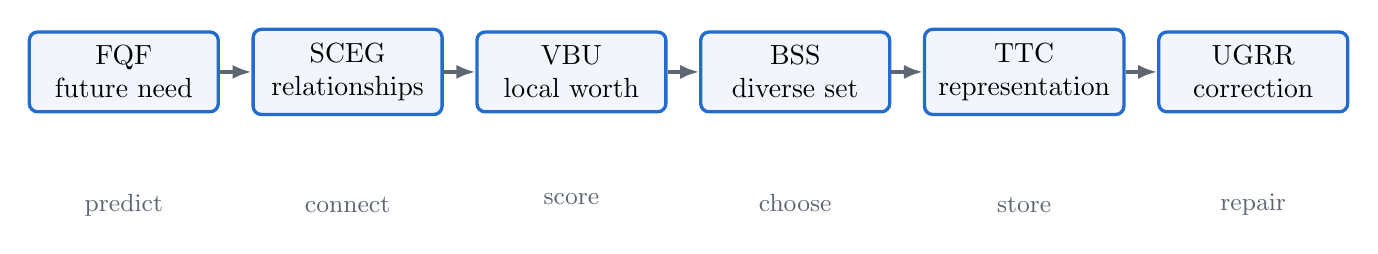
\begin{tikzpicture}[node distance=4mm]
  \node[mainflow, minimum width=2.4cm] (f) {FQF\\future need};
  \node[mainflow, minimum width=2.4cm, right=of f] (g) {SCEG\\relationships};
  \node[mainflow, minimum width=2.4cm, right=of g] (u) {VBU\\local worth};
  \node[mainflow, minimum width=2.4cm, right=of u] (s) {BSS\\diverse set};
  \node[mainflow, minimum width=2.4cm, right=of s] (t) {TTC\\representation};
  \node[mainflow, minimum width=2.4cm, right=of t] (r) {UGRR\\correction};
  \draw[arrow] (f) -- (g);
  \draw[arrow] (g) -- (u);
  \draw[arrow] (u) -- (s);
  \draw[arrow] (s) -- (t);
  \draw[arrow] (t) -- (r);
  \node[note, below=9mm of f] {predict};
  \node[note, below=9mm of g] {connect};
  \node[note, below=9mm of u] {score};
  \node[note, below=9mm of s] {choose};
  \node[note, below=9mm of t] {store};
  \node[note, below=9mm of r] {repair};
\end{tikzpicture}}
\caption{The six MKV responsibilities form one chain. Removing a component creates a named
ablation, not a silent replacement.}
\label{fig:six-chain}
\end{figure}

\subsection{Quality safeguards added around the core chain}

The implementation includes six conservative safeguards:

\begin{enumerate}
  \item \term{Prompt-anchored selection}: PAR keeps a small amount of direct prompt evidence.
  \item \term{Label-free fidelity calibration (LFC)}: configuration candidates are chosen by
        token agreement, logit KL, attention-output error, forecast regret, and actual bytes on a
        disjoint calibration ledger, not by benchmark labels.
  \item \term{Per-head routing (PHR)}: stable/shifted forecast heads receive different prompt/draft
        mixtures, and prototype-sensitive heads receive ET or smaller PT clusters.
  \item \term{Fine evidence preservation}: EPR reserves local structured evidence.
  \item \term{RoPE-safe PT}: the PKT merges keys only in phase-neutral space.
  \item \term{Decision-aware repair}: DAR uses prototype risk plus token margin and can disable
        itself if calibration is not precise enough.
\end{enumerate}

\why These safeguards target observed classes of failure without changing model weights or tuning
on evaluation labels. They still need held-out, clean-worktree experimental validation before any
general quality claim.

\section{A complete worked example}
\label{sec:example}

\begin{plainbox}{Teaching example only}
All values in this section are imaginary round numbers chosen to explain the algorithm. They are
not measured results and must not appear in a measured-results table.
\end{plainbox}

Imagine one layer/head has 16 source positions and block size $b=4$. It therefore has four source
blocks: $B_0=[0,1,2,3]$, $B_1=[4,5,6,7]$, $B_2=[8,9,10,11]$, and
$B_3=[12,13,14,15]$. Suppose $B_3$ contains the generation marker and is mandatory.

The active budget can hold two exact blocks plus one one-slot prototype. Follow the pipeline:

\begin{enumerate}
  \item \term{FQF}: a two-step draft predicts strong future attention on positions 6 and 10.
  \item \term{SCEG}: layout metadata connects $B_1$ (row label) with $B_2$ (numeric cell); $B_0$
        is mostly unrelated decoration.
  \item \term{VBU}: $B_2$ has the highest expected output contribution, $B_1$ is novel, and
        $B_3$ is mandatory.
  \item \term{BSS}: select $B_3$ first, then $B_2$. The budget cannot hold another exact block
        plus the required PT slot.
  \item \term{TTC}: keep $B_2$ and $B_3$ in ET. Assign compatible unselected $B_1$ to anchor
        $B_2$ and make one PT summary. Store original $B_1$ in RT. If $B_0$ has no safe anchor,
        construction must either find a feasible exact-only plan or fail closed; it cannot claim a
        complete PT representation while silently dropping it.
  \item \term{UGRR}: at decode step 3, imagine the model has low decision margin and high attention
        on the $B_1$--$B_2$ prototype. Restore $B_1$, promote it to ET, refresh or remove its PT,
        and recompute step 3 once.
\end{enumerate}

\begin{figure}[htbp]
\centering
\resizebox{0.96\textwidth}{!}{%
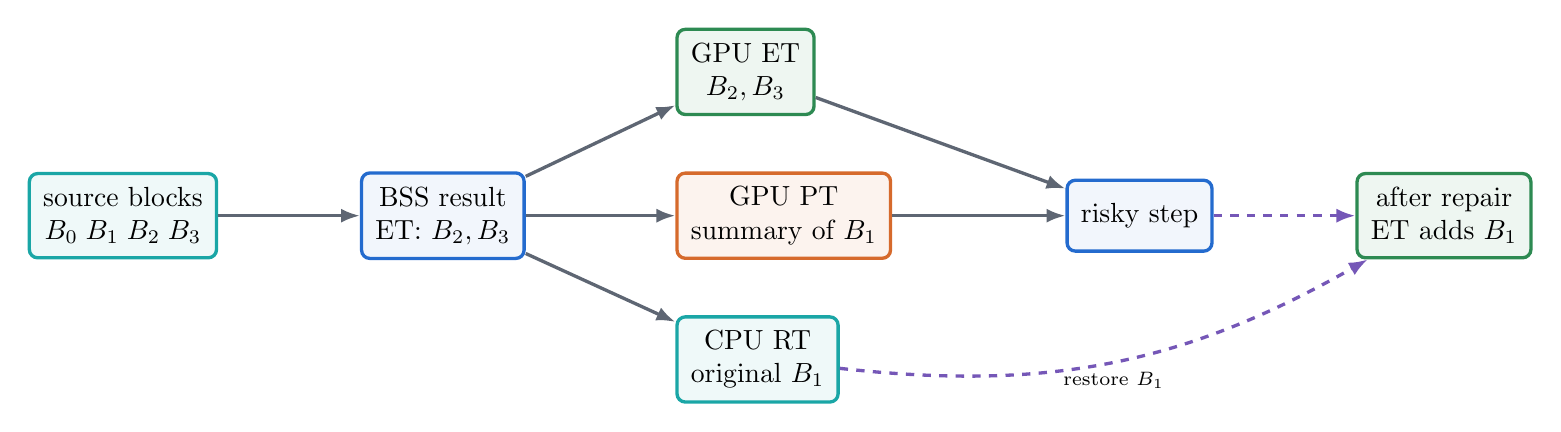
\begin{tikzpicture}[node distance=8mm and 18mm]
  \node[dataflow] (source) {source blocks\\$B_0\;B_1\;B_2\;B_3$};
  \node[mainflow, right=of source] (selected) {BSS result\\ET: $B_2,B_3$};
  \node[safe, above right=7mm and 19mm of selected] (et) {GPU ET\\$B_2,B_3$};
  \node[warn, right=19mm of selected] (pt) {GPU PT\\summary of $B_1$};
  \node[dataflow, below right=7mm and 19mm of selected] (rt) {CPU RT\\original $B_1$};
  \node[mainflow, right=22mm of pt] (risk) {risky step};
  \node[safe, right=of risk] (after) {after repair\\ET adds $B_1$};
  \draw[arrow] (source) -- (selected);
  \draw[arrow] (selected) -- (et);
  \draw[arrow] (selected) -- (pt);
  \draw[arrow] (selected) -- (rt);
  \draw[arrow] (et) -- (risk);
  \draw[arrow] (pt) -- (risk);
  \draw[dashedarrow] (risk) -- (after);
  \draw[dashedarrow] (rt) to[bend right=18] node[below,tinylabel] {restore $B_1$} (after);
\end{tikzpicture}}
\caption{One fictional request from blockization through repair.}
\label{fig:toy}
\end{figure}

The example shows why \term{active bytes} and \term{residual bytes} must be reported separately.
ET and PT occupy active GPU KV. RT occupies CPU memory and adds potential transfer/re-decode cost.

\section{Three public MosaicKV (MKV) methods}
\label{sec:methods}

The unified runtime exposes three MKV methods. They share FQF, SCEG, VBU, BSS, the same block size,
and the same byte accounting.

\begin{table}[htbp]
\centering
\small
\begin{tabularx}{\textwidth}{>{\bfseries}p{0.20\linewidth}c c c X}
\toprule
Method & ET selection & PT merge & RT/UGRR & Meaning \\
\midrule
\code{mosaickv_exact} & yes & no & no & Forecasted graph-aware whole-block selection only. \\
\code{mosaickv_proto} & yes & yes, if safe & no & ET plus position-safe PT summaries. \\
\code{mosaickv_full} & yes & yes, if safe & yes, if safe & Complete ET/PT/RT design with configured UGRR. \\
\bottomrule
\end{tabularx}
\caption{Public MKV methods. An unsafe prototype path receives an explicit exact-only fallback
label, so a fallback row cannot be mistaken for PT or UGRR evidence.}
\label{tab:methods}
\end{table}

\why Separate methods make ablation and debugging clear. If exact selection fails, prototypes
cannot hide the problem. If PT works but repair is costly, \code{mosaickv_proto} isolates that
trade-off.

\section{How MosaicKV (MKV) differs from baselines (BLs)}
\label{sec:baselines}

A baseline (BL) is a comparison method. Fair comparison means all methods receive identical model
weights and precision, processor, media preprocessing, prompt, output length, greedy decoding,
active KV byte budget, mandatory policy, block granularity where applicable, attention backend,
warmups, and measurement protocol.

\begin{longtable}{>{\raggedright\arraybackslash}p{0.20\linewidth}p{0.30\linewidth}p{0.41\linewidth}}
\toprule
Method & Main idea & Key difference from MKV \\
\midrule
\endhead
FullKV & Keep every K/V entry unchanged. & Ground truth; no compression, PT, RT, or UGRR. \\
Random KV & Randomly retain nonmandatory blocks under the same recorded seed and byte budget. & No
attention, value, graph, or forecast signal. \\
Uniform KV & Retain the same fraction in each layer/head/modality. & Enforces even allocation but
does not follow request-specific evidence. \\
Prompt Attention Top-$k$ & Rank blocks using prompt-window attention mass only. & No draft future
signal, value novelty, SCEG coverage, PT, or UGRR. \\
Value Top-$k$ & Rank using value novelty only. & Ignores predicted attention and set coverage. \\
\code{lookm_reimpl} & Local paper-faithful LOOK-M reimplementation with text-prior scoring, pivots,
and its own merge rules. & Its scoring and merging remain distinct; it is not official LOOK-M. \\
\code{prefixkv_reimpl} & Local paper-faithful PrefixKV reimplementation using layer-wise prefix
budgets from an offline profile. & Allocates by layer prefix rather than request-specific SCEG/VBU. \\
\code{vl_cache_reimpl} & Local reimplementation of the ICLR VL-Cache method using modality-aware
sparsity and layer-adaptive calibration. & Uses its paper-derived modality/layer policy, not MKV's
FQF/SCEG/TTC; no official implementation is claimed. \\
MKV exact & FQF + SCEG + VBU + BSS with ET only. & Request-specific future and evidence-aware
selection. \\
MKV prototype & MKV exact plus safe PT. & Represents compatible omissions inside the active
budget. \\
MKV full & MKV prototype plus RT and UGRR/DAR. & Can revise a compression decision during decode. \\
\bottomrule
\end{longtable}

\why These baselines answer different questions. Random KV tests whether intelligent selection
matters. Prompt Attention Top-$k$ tests whether the extra FQF/SCEG/VBU machinery adds value.
Published-method reimplementations compare against closer research ideas, while their
implementation provenance remains explicit.

\begin{plainbox}{Budget rule}
Do not compare methods only by a label such as ``20\% tokens retained.'' Compare the measured ET
+ PT active KV bytes. Report RT bytes separately. If two methods cannot use the same accounting
boundary, they do not belong in directly comparable rows.
\end{plainbox}

\section{Fidelity calibration without answer-label tuning}
\label{sec:calibration}

Label-free fidelity calibration (LFC) chooses among a small preregistered set of MKV
configurations. Each candidate must run on the same calibration sample identifiers (IDs) and
remain under the same measured active-byte ceiling.

For calibration observation $x$, the implementation forms the loss

\begin{equation}
  L_x=(1-A_{tok})+\log(1+D_{KL})+E_{attn}+R_{forecast},
\end{equation}

where $A_{tok}$ is token agreement with FullKV, $D_{KL}$ is logit Kullback--Leibler (KL)
divergence, $E_{attn}$ is attention-output error, and $R_{forecast}$ is forecast regret. Candidate
cost is mean loss plus a weighted 90th-percentile tail loss. Bootstrap resampling checks whether
the same candidate is selected often enough.

\why Final benchmark score alone is a weak calibration target and can leak task answers. LFC uses
internal FullKV fidelity signals and separate calibration/evaluation ledgers. It favors stable
behavior, not only the mean of a tiny sample.

\safety Calibration and evaluation sample IDs must be disjoint. Every candidate must cover the
same calibration ledger. The chosen parameters and profile secure hash algorithm identifier (SHA)
are frozen before held-out evaluation.

\section{Cache materialization and decode mechanics}
\label{sec:materialization}

\subsection{Dense physical capacity}

Many Hugging Face (HF) cache implementations use dense tensors. Even if one layer/head logically
selects fewer positions, physical storage may be determined by the largest packed length. The HF
runtime therefore resolves a \term{dense physical cache budget (DPCB)} before selection. It
quantizes the requested byte target to a representable capacity and enforces per-layer/head
position limits.

\why Counting logical selected blocks while allocating a larger dense tensor would under-report
real active memory. DPCB ensures the selector's budget matches the actual packed storage boundary.

\subsection{Packing exact and prototype slots}

Within each layer/head, ET entries are sorted by original logical position. PT entries occupy
their anchor logical positions. If every packed position is valid and all layer/head capacities
match, decode can use an all-valid fast path. If lengths differ, the eager runtime builds checked
validity masks and supplies per-layer attention masks.

The next generated token is appended physically after the packed prompt but receives the original
next logical position. Generated positions advance from the logical prompt length, not packed
length.

\safety Packed K/V tensors, masks, prefill logits, and decode logits are checked for not-a-number
(NaN) or infinity. A compressed state without a valid logical-position mask is rejected.

\subsection{Explicit deterministic decoding}

Temperature is zero, sampling is disabled, and each token is selected by deterministic
\code{argmax}. The first token comes from the prefill logits. Later tokens use
\code{decode_one_token}. Terminal-token rules and maximum output length are shared across FullKV,
MKV, and baseline (BL) methods.

\why Deterministic decoding makes parity failures reproducible and prevents random generation
noise from being confused with a compression effect.

\section{Measurement and provenance implementation}
\label{sec:measurement}

Performance and quality results are useful only when their origins are inspectable. MKV writes an
immutable run manifest, structured JavaScript Object Notation (JSON) logs, raw JSON Lines (JSONL)
sample records, aggregate Apache Parquet files, and one debug trace per attempted sample.

\subsection{Timing boundaries}

On a GPU, timing uses \code{torch.cuda.Event} and calls \code{torch.cuda.synchronize} at timing
boundaries. The runtime separates:

\begin{itemize}
  \item image/video encoder time;
  \item multimodal projector time;
  \item language-model (LM) prefill time;
  \item FQF, SCEG, VBU/BSS, TTC, and total compression time;
  \item time to first token (TTFT);
  \item per-token and total decode time, which yield inter-token latency (ITL);
  \item RT transfer and re-decode repair time; and
  \item end-to-end (E2E) latency.
\end{itemize}

Repeated trials retain every raw observation and derive median, 5th percentile (p5), 95th
percentile (p95), mean, standard deviation (SD), and bootstrap confidence intervals (CIs).

\why GPU work is asynchronous. A host clock can stop before the GPU finishes, producing falsely
small latency. CUDA events and synchronization make timing boundaries explicit.

\subsection{Memory accounting}

The runtime records:

\begin{itemize}
  \item \code{torch.cuda.max_memory_allocated};
  \item \code{torch.cuda.max_memory_reserved};
  \item active ET/PT KV bytes from tensor element counts and dtype size;
  \item CPU RT bytes from the actual residual encoding; and
  \item repaired/restored bytes per event.
\end{itemize}

Active bytes are computed from underlying tensor storage. Metadata is not silently counted by one
method and ignored by another. The accounting boundary is written into the configuration and
trace.

\subsection{Required manifest fields}

Every experimental row resolves to:

\begin{itemize}
  \item Git SHA, configuration SHA, and dirty-worktree state/patch identity;
  \item model ID/revision and dataset ID/revision;
  \item Compute Unified Device Architecture (CUDA), driver, PyTorch, Transformers, vLLM, and
        SGLang versions;
  \item GPU type/count, power and clock state, and background GPU processes;
  \item backend, attention implementation, model precision, and process concurrency;
  \item seed, output policy, and measurement type; and
  \item prompt/media/tokenization and generation identities needed for paired comparison.
\end{itemize}

\why Without these fields, a row cannot be reproduced or compared fairly. A dirty-worktree run is
exploratory even if its patch is preserved.

\subsection{Debug trace}

The MKV trace includes FQF statistics, predicted attention provenance, SCEG typed edges, every VBU
signal, BSS marginal gains/reasons, ET/PT/RT membership, PKT provenance, packed positions,
repair events, token IDs, bytes, and timing. A failed sample writes an explicit error row and trace
instead of disappearing.

\why An answer alone cannot explain why compression succeeded or failed. The trace lets a
researcher inspect the selected evidence and the exact point at which a fallback or repair occurred.

\section{Correctness invariants and tests}
\label{sec:tests}

An invariant is a rule that must always be true. The implementation checks these invariants in
dataclass construction, runtime planning, unit tests, property-based tests (PBTs), and real-model
gates.

\begin{longtable}{>{\bfseries}p{0.08\linewidth}p{0.54\linewidth}p{0.30\linewidth}}
\toprule
ID & Invariant & Why it matters \\
\midrule
\endhead
I1 & Every source cache position belongs to exactly one KVBD in its layer/head. & Prevents missing
or double-counted source data. \\
I2 & ET membership never conflicts with PT/RT source membership; PT and RT overlap only by the
declared recovery relationship. & Prevents contradictory ownership. \\
I3 & Active-byte accounting equals ET/PT tensor storage. & Enforces the real budget. \\
I4 & Retention 1.0 reconstructs FullKV exactly with empty PT/RT. & Establishes the identity path. \\
I5 & Mandatory blocks remain ET. & Protects causal/control tokens. \\
I6 & Logical positions are monotonic inside every block. & Preserves positional meaning. \\
I7 & DR leaves the original prefill cache and state unchanged. & Prevents forecast tokens from
leaking into final decoding. \\
I8 & BSS is deterministic and never exceeds its budget. & Makes runs reproducible and fair. \\
I9 & PT never mixes layers/heads or incompatible RoPE phases. & Avoids invalid summaries. \\
I10 & UGRR re-decodes a triggered step at most once and keeps the active budget valid. & Bounds
latency and state mutation. \\
I11 & Policy \code{none} produces zero repair events. & Establishes the no-repair control. \\
I12 & Online FQF/UGRR cannot import evaluation-only oracle decisions. & Prevents future-information
leakage. \\
\bottomrule
\end{longtable}

\subsection{Test levels}

\begin{enumerate}
  \item \term{CPU unit tests}: strict configuration, synthetic tensors, graph edges, formulas,
        budget rules, exact/prototype construction, RT round trips, and repair state transitions.
  \item \term{PBTs}: random tensor shapes, block sizes, position maps, and selector conditions.
  \item \term{GPU smoke tests}: CUDA paths, pinned memory, asynchronous transfer, and tiny matrix
        operations without downloading large model weights.
  \item \term{Checkpoint parity tests}: explicit FullKV loop versus ordinary generation, extraction
        and reinjection, and retention-1.0 MKV for at least 16 greedy tokens.
  \item \term{Dataset progression}: small fixed ledgers before any full benchmark campaign.
\end{enumerate}

\why A synthetic test can prove an equation or state invariant, but only a real checkpoint can
prove model-specific cache compatibility. A small checkpoint test can prove execution, but only a
clean, sufficiently sized benchmark can support a scientific performance claim.

\section{Configuration and command-line use}
\label{sec:configuration}

Behavior-affecting choices live in strict versioned YAML configuration. Unknown fields and invalid
combinations fail with useful messages. The following example illustrates the structure; it is not
a recommended paper configuration and uses placeholders for immutable revisions.

\begin{lstlisting}[style=mosaickv,language={}]
schema_version: 1
model:
  id: Qwen/Qwen2.5-VL-3B-Instruct
  revision: MODEL_COMMIT_SHA
  precision: bf16
dataset:
  id: synthetic_smoke
  revision: DATASET_REVISION
execution:
  backend: huggingface
  attention_implementation: eager
  seed: 2027
generation:
  max_new_tokens: 32
  temperature: 0.0
  do_sample: false
cache:
  block_size: 16
  retention_ratio: 0.40
  budget_unit: bytes
method: mosaickv_full
forecasting:
  mode: hybrid
  prompt_window: 16
  draft_steps: 4
  centroid_count: 4
  low_memory_centroids: true
graph:
  max_neighbors: 8
  similarity_chunk_size: 256
selection:
  algorithm: lazy_greedy
  prompt_anchor_fraction: 0.05
  evidence_preservation_fraction: 0.05
prototypes:
  enabled: true
  group_size: 4
  max_position_span: 128
residual:
  enabled: true
  storage_dtype: lossless
  require_pinned_memory: true
repair:
  enabled: true
  policy: decision_aware
  max_blocks_per_step: 1
\end{lstlisting}

The command-line interface (CLI) can run the same shape directly:

\begin{lstlisting}[style=mosaickv,language={}]
source mosaickv/scripts/cache_env.sh
/scratch/djy8hg/env/mosaickv/bin/mosaickv evaluate \
  --model Qwen/Qwen2.5-VL-3B-Instruct \
  --backend hf \
  --attention-backend eager \
  --method mosaickv_full \
  --task synthetic_smoke \
  --retention-ratio 0.4 \
  --block-size 16 \
  --forecast hybrid \
  --draft-tokens 4 \
  --repair-policy decision_aware
\end{lstlisting}

All caches and temporary files must remain under \code{/scratch/djy8hg}, normally
\code{/scratch/djy8hg/cache/mosaickv}; the home directory is not used for package, HF, dataset,
compiler, or temporary caches. The HF token (\code{HF_TOKEN}) is accepted only through the process
environment and is never written into project files or manifests.

\section{Implementation map}
\label{sec:implementation-map}

This table connects each concept to the actual Python source. Paths are relative to
\code{mosaickv/}.

\begin{longtable}{>{\raggedright\arraybackslash}p{0.25\linewidth}p{0.33\linewidth}p{0.33\linewidth}}
\toprule
Concept & Main source & Key types/functions \\
\midrule
\endhead
Strict configuration & \code{src/mosaickv/config.py}, \code{types.py} & \code{RunConfig}, component
configs, controlled enums, canonical config SHA \\
Adapter interface & \code{src/mosaickv/adapters/huggingface/} & \code{AdapterCapabilities},
\code{DecodeState}, model-family adapters \\
FullKV reference & \code{src/mosaickv/fullkv.py} & \code{FullKV}, synchronized trial runner \\
Cache state/blockization & \code{src/mosaickv/cache_state.py} & \code{KVBlockDescriptor},
\code{LogicalPositionMap}, \code{FullKVState}, \code{MosaicKVState} \\
FQF & \code{src/mosaickv/forecasting/} & \code{QueryForecast},
\code{forecast_with_rollout}, deterministic centroids \\
SCEG & \code{src/mosaickv/graph/} & \code{SparseEvidenceGraph},
\code{build_evidence_graph}, pooling and diagnostics \\
VBU & \code{src/mosaickv/selection/utility.py} & \code{compute_block_utilities},
\code{BlockUtilityTable} \\
BSS & \code{src/mosaickv/selection/} & \code{BudgetedObjective},
\code{lazy_greedy_select}, exhaustive solver \\
LFC/PHR & \code{src/mosaickv/selection/calibration.py} & fidelity profile selection and adaptive
head routing \\
ET/PT/RT construction & \code{src/mosaickv/prototypes/}, \code{residual/} &
\code{construct_three_tier_cache}, prototype records, residual storage \\
PKT & \code{src/mosaickv/prototypes/rope.py} & \code{RotaryPrototypeKeyTransform} \\
UGRR/DAR & \code{src/mosaickv/repair/} & \code{RepairCacheState},
\code{repair_decode_step}, calibration and oracle isolation \\
Unified HF runtime & \code{src/mosaickv/backends/hf_runtime.py} &
\code{HuggingFaceMosaicKVModel}, compression plan, packing, explicit decode \\
Measurements & \code{src/mosaickv/measurements/} & CUDA timers, byte accounting, telemetry,
trial statistics \\
Evaluation/results & \code{src/mosaickv/evaluation/} & task registry, local model adapter, JSONL,
Parquet, resume and merge \\
Provenance/logging & \code{src/mosaickv/manifest.py}, \code{logging.py} & run manifest and structured
JSON logging \\
\bottomrule
\end{longtable}

\section{Current model and backend support}
\label{sec:status}

This section reports the implementation boundary documented in the repository at this document's
snapshot date. ``Implemented'' is not the same as ``paper-validated.'' A paper-ready row still
requires a clean worktree, immutable revisions, passed parity gates, and a controlled measured run.

\subsection{Hugging Face model adapters}

\begin{table}[htbp]
\centering
\small
\begin{tabularx}{\textwidth}{>{\raggedright\arraybackslash}p{0.22\linewidth}c c c X}
\toprule
Model family & Exact HF & RoPE-safe PT & UGRR & Boundary \\
\midrule
Qwen2.5-VL & \mksupported & \mkconditional & \mkconditional & M-RoPE PKT; PT/UGRR require audited
Transformers 4.55.2 eager path and supported position layout. \\
LLaVA-1.5 & \mksupported & \mkconditional & \mkconditional & Standard Llama RoPE PKT; same pinned eager and
monotonic-position restrictions. \\
LLaVA-OneVision & \mksupported & \mkconditional & \mkconditional & Standard Qwen2 RoPE PKT; checkpoint-specific
parity remains required. \\
InternVL2.5 & \mkconditional & \mkunsupported & \mkunsupported & Optional remote-code adapter and checkpoint-specific
preprocessing; exact-only when load-compatible. \\
\bottomrule
\end{tabularx}
\caption{Source-level HF support. ``Conditional'' means the runtime checks and fails closed when
the audited requirements are not met.}
\label{tab:model-support}
\end{table}

\subsection{Attention implementations}

HF FullKV supports eager attention, scaled dot-product attention (SDPA), and FlashAttention-2
(FA2) where the adapter and installed environment declare them. SCEG/VBU selection that requires
explicit attention is prepared through eager attention. PT and UGRR currently require the owned
eager path. Fused PT/UGRR paths are unsupported until cache/mask parity is proven.

An all-valid exact cache can optionally switch to an audited faster decode attention
implementation, but the switch and both prefill/decode implementations must be recorded. A
padded per-head cache or live repair path fails closed rather than silently using an incompatible
kernel.

\subsection{vLLM and SGLang}

vLLM and SGLang FullKV measurement wrappers exist for supported checkpoints. Version-pinned
whole-block transport tests have exercised retention-1.0 identity, partial physical block release,
logical decode positions, and request isolation. However, the repository still blocks compressed
paper-method rows until the common MKV selector-plan bridge is verified end to end.

Serving-backend PT injection and UGRR remain unsupported. A transport test using a fallback
selector is not labeled native MKV.

\why Serving engines jointly manage physical KV ownership, block tables, scheduler state, prefix
or Radix cache metadata, and logical positions. Updating only the K/V tensor would leave the
engine internally inconsistent. The source therefore requires an atomic transaction or fails
explicitly.

\subsection{Honest evidence boundary}

The repository contains exploratory GPU and small-dataset validation, including real PT/UGRR paths
for supported HF adapters. The repository documentation also records negative findings and
calibration gates that disabled unhelpful repair. These runs demonstrate implementation behavior,
not universal superiority or paper-eligible measurements. The current dirty worktree makes new
validation exploratory until the user explicitly requests a clean commit and canonical rerun.

\section{Known limitations and risks}
\label{sec:limitations}

\begin{enumerate}
  \item \term{Compression overhead}: FQF, SCEG, BSS, PKT, packing, and UGRR cost time. Short outputs
        may finish before decode savings repay that cost.
  \item \term{Forecast error}: a short DR can miss evidence needed much later in the answer.
  \item \term{Metadata gaps}: OCR/layout/spatial/temporal edges are only as good as the available
        processor and dataset metadata.
  \item \term{Prototype approximation}: even RoPE-safe averaging can blur two content vectors that
        should remain distinct.
  \item \term{Repair precision}: UGRR can trigger on an uncertain but already correct token. DAR
        calibration may therefore disable repair.
  \item \term{Dense cache limits}: logical selection does not always translate into equal physical
        memory savings on dense HF layouts.
  \item \term{Backend ownership}: serving engines do not yet support full native MKV TTC/UGRR
        transactions.
  \item \term{Model specificity}: PKTs are architecture- and version-specific. New models need new
        source inspection and parity evidence.
  \item \term{Residual memory}: RT reduces active GPU KV but still consumes CPU memory and can add
        transfer/conversion cost.
  \item \term{Evidence status}: small or dirty-tree experiments cannot prove general accuracy or a
        fixed performance advantage over BL methods.
\end{enumerate}

\section{How to reason about a MosaicKV result}
\label{sec:reading-results}

When reading a future MKV result, ask these questions in order:

\begin{enumerate}
  \item Did retention 1.0 pass FullKV token/logit parity for this exact model, revision, precision,
        backend, and attention implementation?
  \item Did compared methods use identical prompts, media, processor, output length, and decoding?
  \item Are budgets actual active KV bytes rather than unmatched nominal retention ratios?
  \item Does the method label reveal an exact-only fallback, or did real PT/RT/UGRR run?
  \item Are compression and repair overhead included in E2E latency?
  \item Are RT bytes reported separately from active bytes?
  \item Are task scores official and per-task, rather than mixed into an unexplained average?
  \item Are every failed sample, seed, and trial retained?
  \item Does the manifest identify a clean Git SHA and immutable model/dataset revisions?
  \item Is the conclusion supported by CIs and held-out examples?
\end{enumerate}

\why MKV is a multi-stage research system. A single score cannot reveal whether a gain came from
better selection, a larger real byte budget, a different prompt, a fallback, or measurement noise.

\section{Summary for a young reader}

Think of a VLM's KV cache as a very large school notebook used while answering a question about a
picture:

\begin{itemize}
  \item FQF guesses which notes the next answer sentences may need.
  \item SCEG draws lines between notes that explain the same fact.
  \item VBU gives each note a usefulness score.
  \item BSS packs a small backpack with useful notes that cover different facts.
  \item TTC keeps the best notes exactly, makes safe summaries of some other notes, and leaves
        recoverable originals in a desk drawer.
  \item UGRR opens the drawer only when the model seems uncertain and a summary looks risky.
\end{itemize}

The hard part is not merely deleting memory. The hard part is preserving the model's original
positions, respecting layer/head boundaries, building only mathematically safe summaries, never
exceeding the same byte budget used by competitors, and recording enough evidence to prove what
actually happened.

\appendix

\section{Compact symbol glossary}

\begin{longtable}{>{\bfseries}p{0.16\linewidth}p{0.75\linewidth}}
\toprule
Symbol & Meaning \\
\midrule
\endhead
$q$ & Query vector for a current token. \\
$k_j,v_j$ & Key and value vectors stored for source position $j$. \\
$a_j$ & Attention probability on source position $j$. \\
$o$ & Attention output, a weighted sum of values. \\
$d$ & Attention-head dimension. \\
$b$ & Fixed token block size. \\
$i$ & Block/node identifier. \\
$p_i$ & Forecast attention probability for block $i$. \\
$c_i$ & Expected attention-output contribution of block $i$. \\
$n_i$ & Value novelty/uniqueness of block $i$. \\
$u_i$ & Local VBU score for block $i$. \\
$S$ & Set of selected exact blocks. \\
$F(S)$ & BSS set objective. \\
$C_{FL}(S)$ & SCEG facility-location coverage by $S$. \\
$C_{mod}(S)$ & Modality coverage by $S$. \\
$\Delta(i\mid S)$ & Marginal gain from adding block $i$ to $S$. \\
$\alpha_j$ & Normalized weight of PT member $j$. \\
$\bar{k},\bar{v}$ & Prototype key and value before casting to cache dtype. \\
$H_{norm}$ & Normalized next-token entropy. \\
$A_j,D_j,R_j$ & PT attention mass, dispersion, and risk. \\
$R$ & Maximum RT source blocks restored in one repair event. \\
\bottomrule
\end{longtable}

\section{Design checklist for adding a new model adapter}

\begin{enumerate}
  \item Pin model and processor revisions; inspect the exact public source.
  \item Record architecture, media capabilities, attention implementations, cache class, tensor
        layout, and sequence dimension.
  \item Implement message/media preparation with the checkpoint's own chat template and processor.
  \item Implement one prefill and explicit one-token decode with deterministic greedy output.
  \item Capture Q vectors at \code{q_proj} without modifying weights.
  \item Determine whether cached K is pre-RoPE or post-RoPE from exact source lines.
  \item Implement extraction/reinjection for the actual cache class; keep active/logical/next
        positions separate.
  \item Pass ordinary generation versus explicit FullKV parity for at least 16 tokens.
  \item Pass extraction/reinjection parity and retention-1.0 MKV parity.
  \item Enable PT only after an audited PKT exists and a real TTC parity/safety gate passes.
  \item Enable UGRR only after PT, pinned RT transfer, partial-prototype refresh, one-redecode, and
        budget tests pass.
  \item Add the exact support boundary to the model/backend capability matrices.
\end{enumerate}

\section{Further repository documentation}

The following Markdown (MD) documents provide implementation-specific detail and validation
history:

\begin{itemize}
  \item \code{docs/cache_state.md}
  \item \code{docs/future_query_forecasting.md}
  \item \code{docs/evidence_graph.md}
  \item \code{docs/block_utility_and_selection.md}
  \item \code{docs/three_tier_cache.md}
  \item \code{docs/decode_time_repair.md}
  \item \code{docs/huggingface_adapters.md}
  \item \code{docs/huggingface_runtime.md}
  \item \code{docs/backend_capability_matrix.md}
  \item \code{docs/model_capability_matrix.md}
  \item \code{SCIENTIFIC_INTEGRITY.md}
  \item \code{REPRODUCIBILITY.md}
\end{itemize}

\end{document}
